\chapter{Functional Verification of Sequential Normal Basis Multiplier}
\label{ch:normal}
In order to utilize our traversal algorithm, it is necessary to find out
a sort of suitable circuit benchmarks which is easy to compute its
Gr\"obner basis (GB). From the work of Lv et al. \cite{lv_dissertation},
we learn that arithmetic circuits in Galois field (GF) is
convertible to an ideal of circuit polynomials, and the 
ideal generators form a GB themselves when applying reverse topological
term order. Furthermore, according to the work of Pruss et al.
\cite{tim_dissertation}, with a limited computation complexity,
we can abstract the word-level signature of an arithmetic 
component working in GF. Thus, we consider the possibility 
of applying our traversal algorithm on sequential Galois
field circuits. In each frame, we can use the techniques 
from \cite{tim_dissertation} to abstract the word-level
signature of the combinational logic, which corresponds
to the transition function in our traversal algorithm.
As a result, we manage to find a type of sequential GF multiplier
which we can apply our traversal algorithm to actually 
verify its functional correctness.

\section{Motivation}
\label{sec:normal_motiv}
From the preliminaries (Chapter \ref{ch:prelim}) about FSMs, we learn that the
Moore machine does not rely on inputs for state transitions. 
As depicted in Figure \ref{fig:Moore}(a), a typical Moore machine implementation
consists of combinational logic component and register files, where
$r_0,\dots,r_k$ are present state (PS) variables 
standing for state inputs (SI), and $r_0',\dots,r_k'$ are next state (NS) variables standing for
state outputs (SO). Figure \ref{fig:Moore}(b) shows the state transition graph (STG) of 
a Moore machine with $k+1$ distinct states. We notice that it forms a simple chain,
with $k$ consecutive transitions the machine reaches final state $R_k$.

\begin{figure}[H]
\centering{
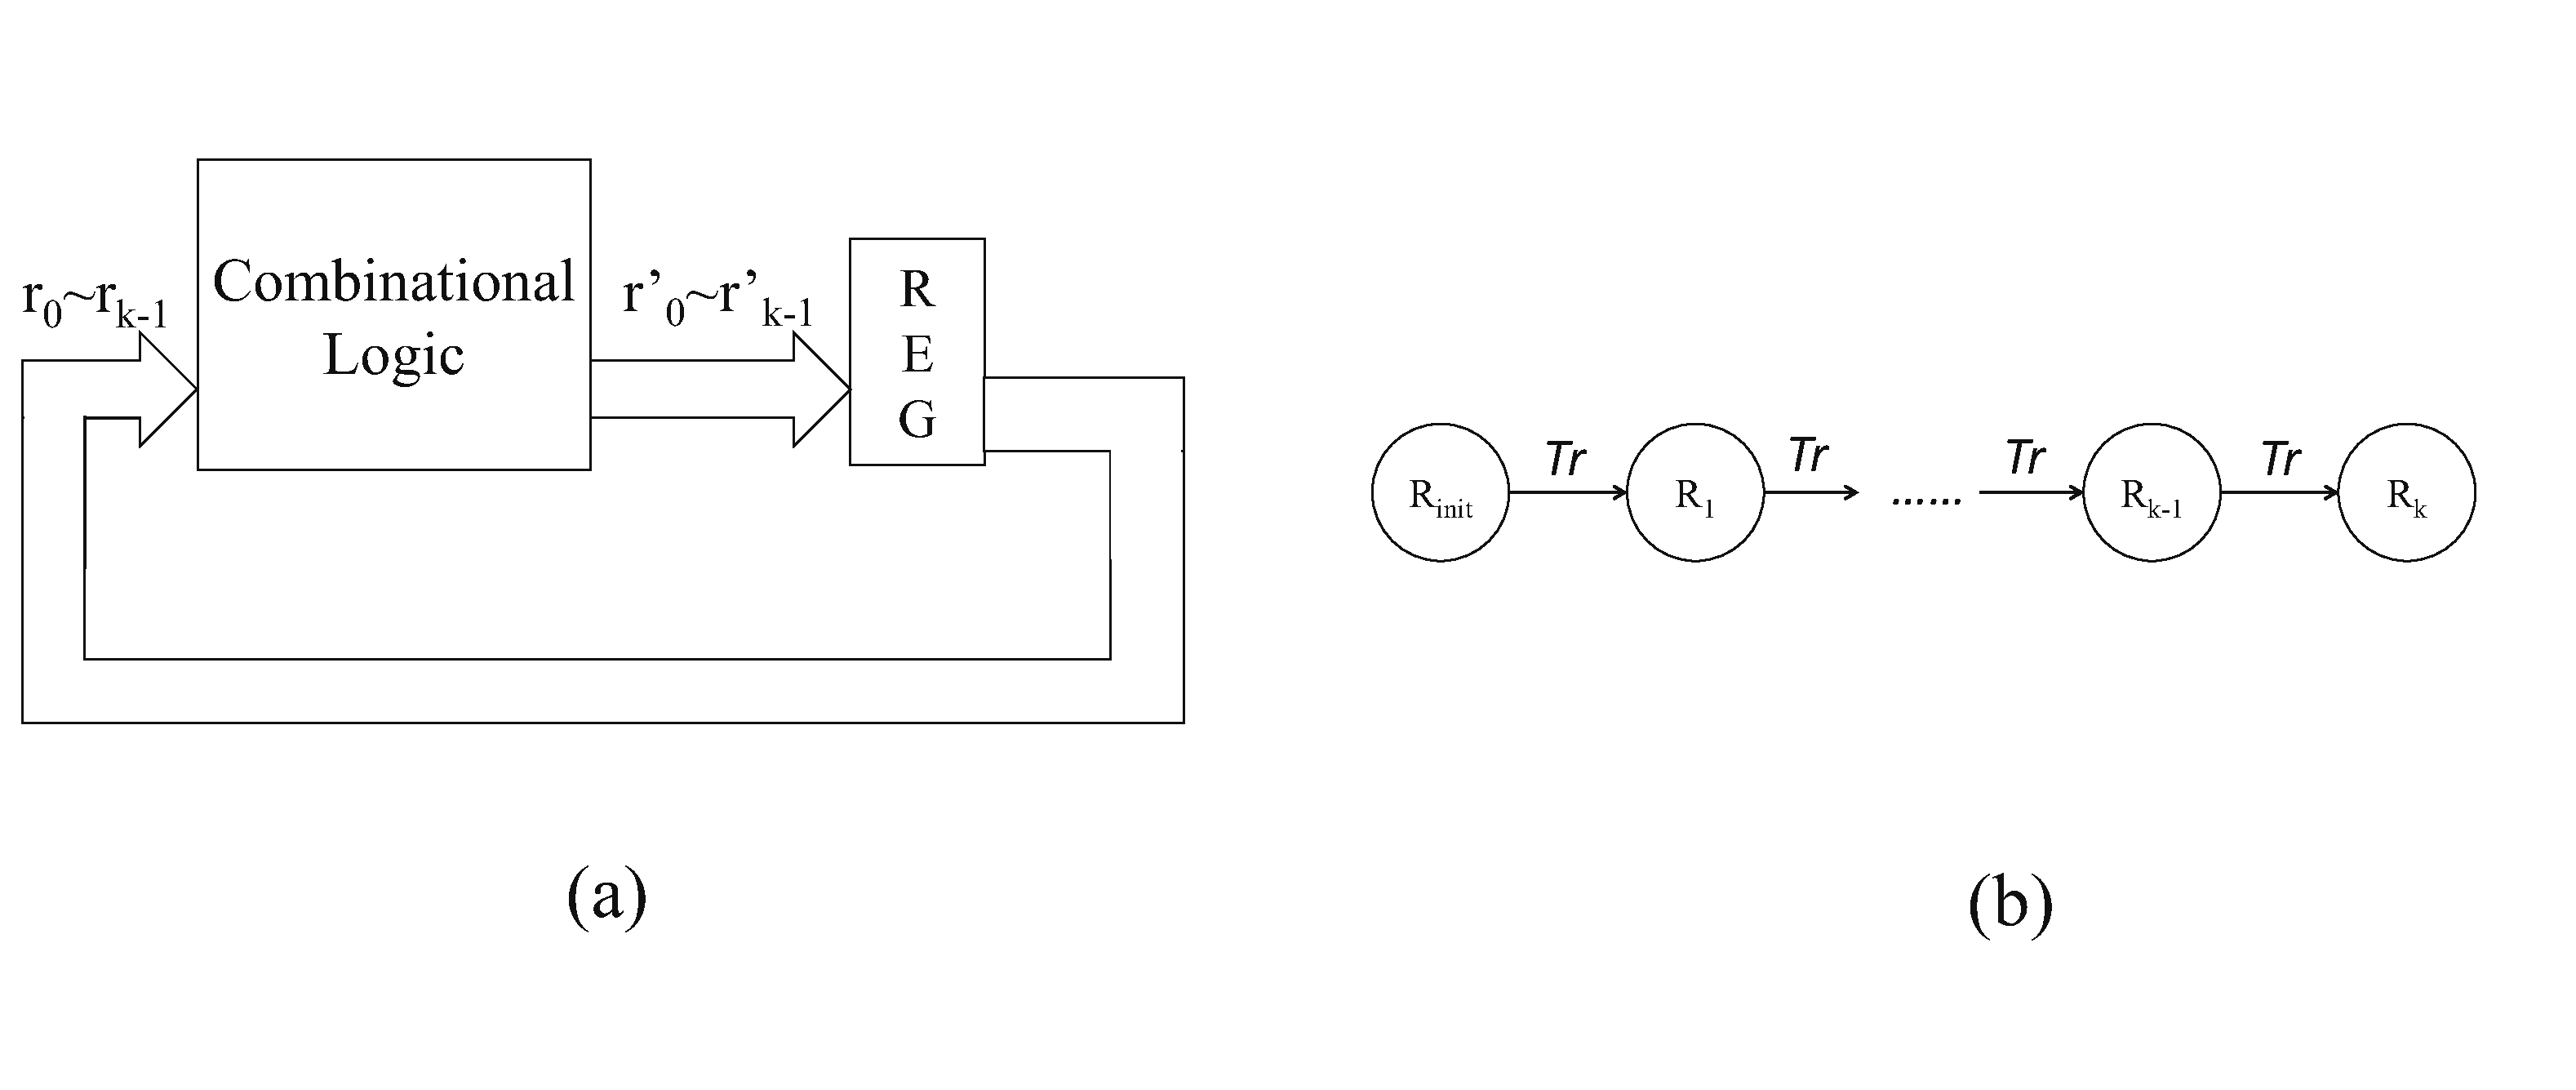
\includegraphics[width=\textwidth]{newfig/Moore.eps}
\caption{A typical Moore machine and its state transition graph}
\label{fig:Moore}}
\end{figure}

In practice,
some arithmetic components are designed in sequential circuits similar to the structure in 
Figure \ref{fig:Moore}(a). Initially the operands are loaded into the registers, 
then the closed circuit executes without taking any additional information from outside,
and store the results in registers after $k$ clock cycles. Its behavior can be described using
STG in Figure \ref{fig:Moore}(b): state $R$ denotes the bits stored in registers. Concretely, $R_init$ is the initial
state (usually reset to all zeros), $R_1$ to $R_{k-1}$ are intermediate results stored as SO of current state and SI
for next state, and $R_k$ (or $R_{final}$) is the final result given by arithmetic circuits (and equals to the answer
to arithmetic function when circuit is working functional correctly).
This kind of design results in 
reusing a smaller combinational logic component such that the area cost is greatly optimized.
However, it also brings difficulties in verifying the the circuit functions.

\begin{figure}[H]
\centering{
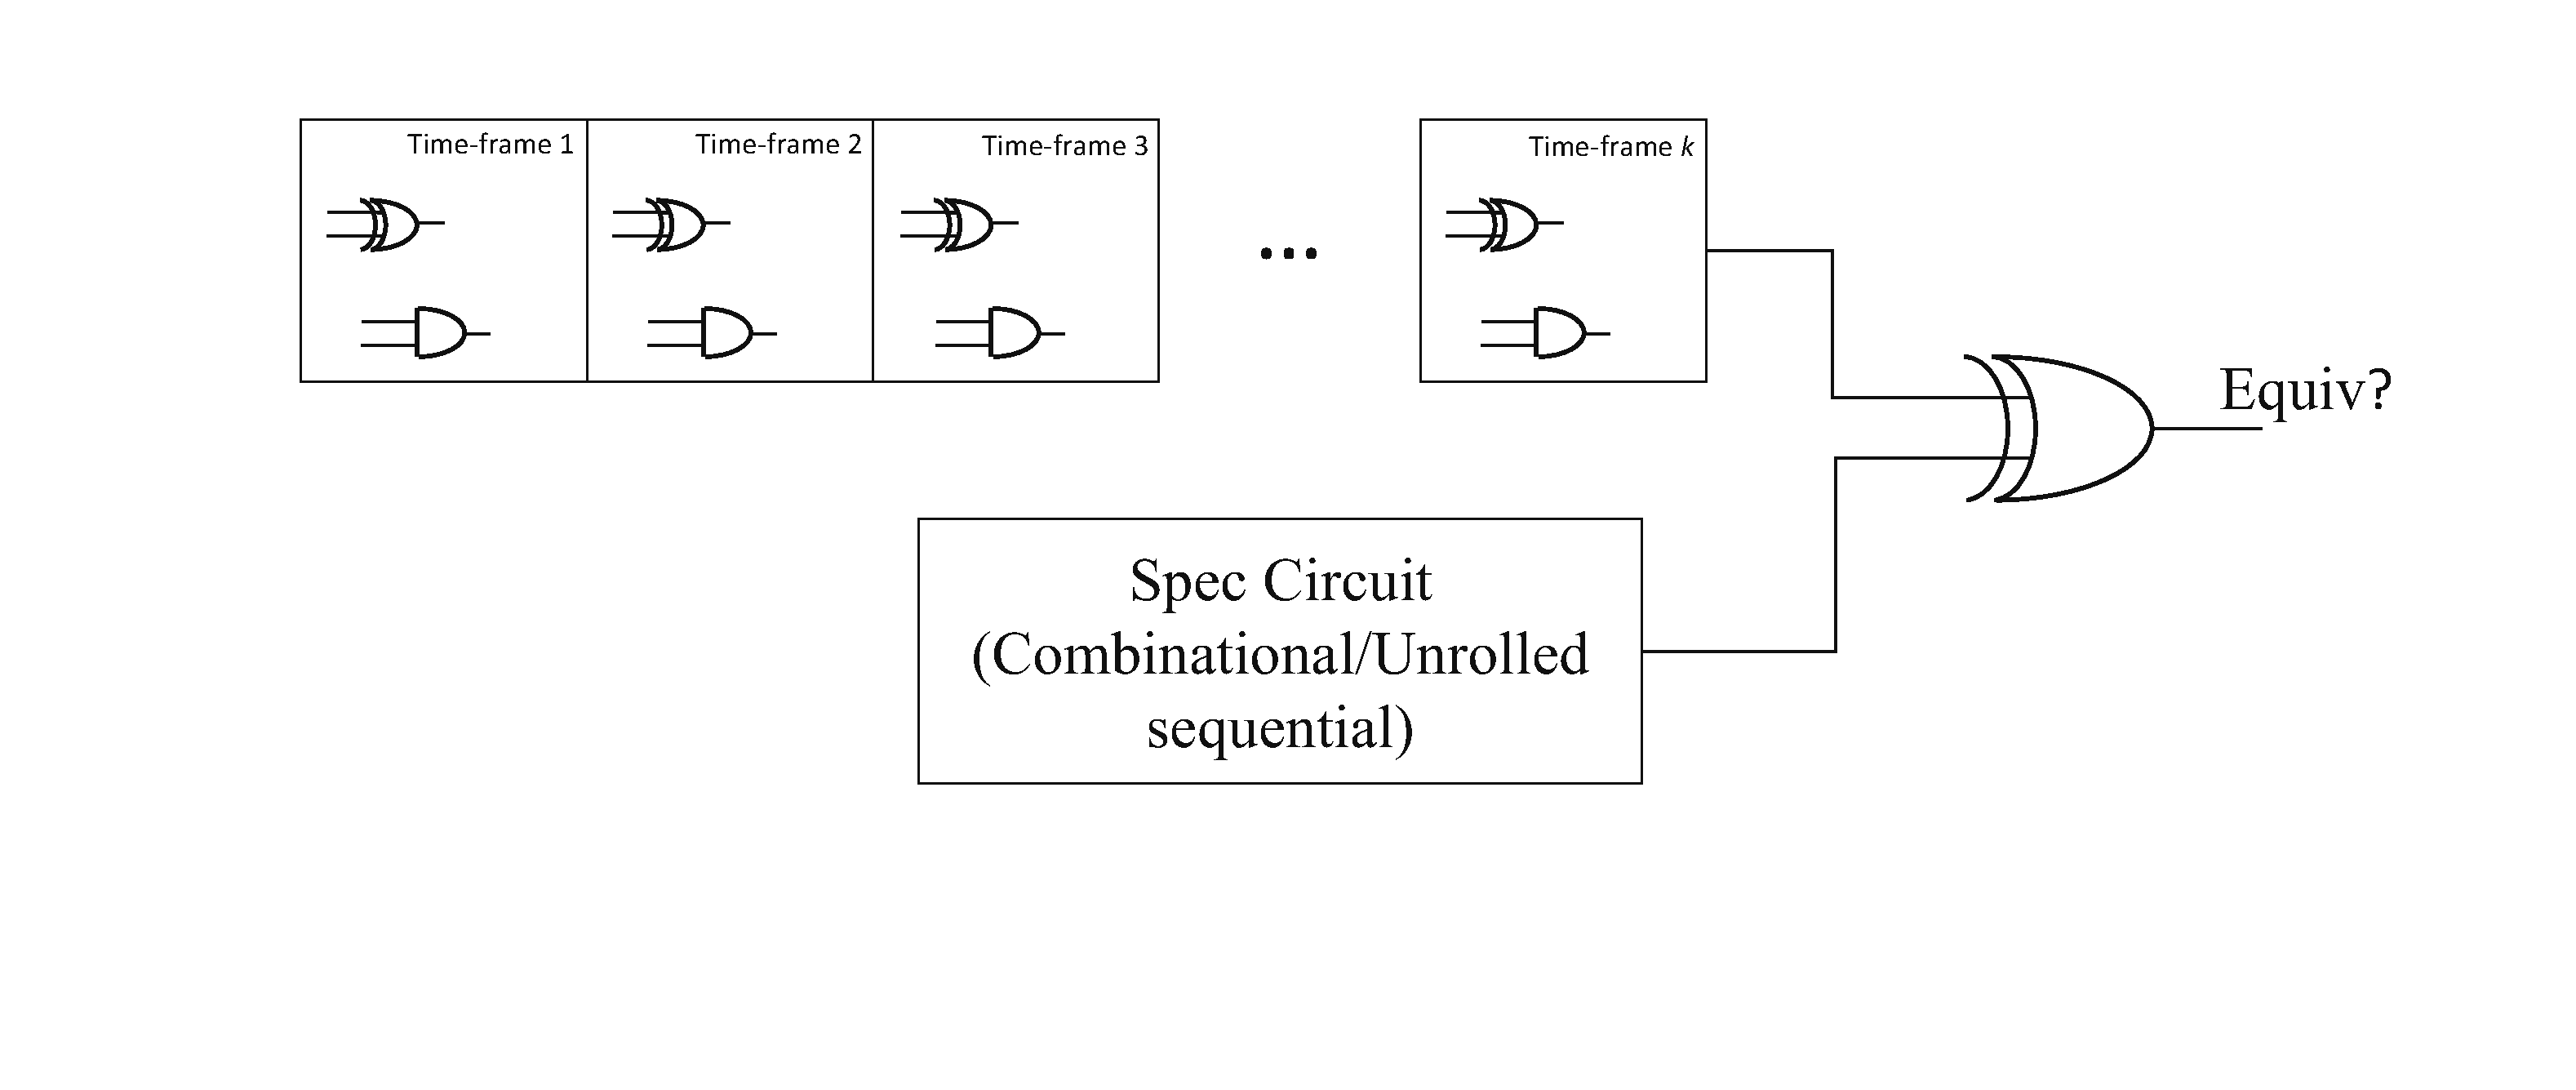
\includegraphics[width=\textwidth]{newfig/convention.eps}
\caption{Conventional verification techniques based on bit-level unrolling and equivalence checking}
\label{fig:convention}}
\end{figure}

Conventional methods to such a sequential circuit may consist of unrolling the circuit for 
$k$ time-frames, and performing an equivalence checking between the unrolled machine and
the specification function. However, the number of gates will grow fast when doing unrolling
on bit-level. Meanwhile the structural similarity based equivalence checking techniques 
will fail when the sequential circuit is highly customized and optimized from the naive specification 
function. As a result, conventional techniques is grossly inefficient for large circuits.
Therefore, a new method based on our proposed word-level FSM traversal technique is worthy to be explored.

\section{Normal Basis Multiplier over Galois Field}
From algebraic view, a field is a space, and field elements are dots in the space. Those elements can be 
represented with unique coordinates, which requires the pre-definition of a basis vector. In this
section, we discuss a special basis called normal basis, as well as the advantages adopting it in 
GF operations esp. multiplication.
\subsection{Normal Basis}
Given a Galois field (GF) $\Fkk$ is a finite field with  $2^k$ elements and characteristic equals to 2.
Its elements can be written in polynomials of $\alpha$, when there is an irreducible polynomial $p(\alpha)$
defined.

If we use a basis $\{1,\alpha,\alpha^2,\alpha^3,\dots,\alpha^{k-1}\}$, we can easily transform polynomial representations
to binary bit-vector representations by recording the coefficients. For example,

\begin{table}[H]
\centering
\caption{Bit-vector, Exponential and Polynomial representation of
elements in  ${\mathbb{F}}_{2^4} = {\mathbb{F}}_2[x]
\pmod{x^4+x^3+1}$}
\begin{tabular}{|c|c||c|c|} 
\hline
$a_3a_2a_1a_0$ & Polynomial     &$a_3a_2a_1a_0$ & Polynomial  \\
\hline
$0000$        & $0$           & $1000$  &$\alpha^3$\\
\hline
$0001$        & $1$           & $1001$  & $\alpha^3 + 1$\\
\hline
$0010$        &  $\alpha$       & $1010$ & $\alpha^3 + \alpha$  \\
\hline
$0011$        &  $\alpha + 1$   & $1011$ &  $\alpha^3+\alpha+1$\\
\hline
$0100$        &  $\alpha^2$     &  $1100$ &  $\alpha^3 + \alpha^2$\\
\hline
$0101$        & $\alpha^2 + 1$ & $1101$  & $\alpha^3+\alpha^2+1$\\
\hline
$0110$        &  $\alpha^2 + \alpha$ & $1110$ &  $\alpha^3+\alpha^2+\alpha$\\
\hline
$0111$        & $\alpha^2+\alpha+1$ & $1111$ & $\alpha^3+\alpha^2+\alpha+1$\\
\hline
\end{tabular}
\label{table:booltogalois}  
\end{table}

Basis $\{1,\alpha,\alpha^2,\alpha^3,\dots,\alpha^{k-1}\}$ is called {\bf standard basis} (StdB), which results in
a straightforward representation for elements, and operations of elements such as addition and subtraction.
The addition/subtraction of GF elements in StdB follows the rules of polynomial addition/subtraction
where coefficients belong to $\mathbb F_2$. In other words, using the definition of {\it exclusive or} (XOR) in
Boolean algebra, element $A$ add/subtract by element $B$ in StdB is defined as
\begin{align}\label{eqn:StdB}
A+B = A-B &= (a_0,a_1,\dots,a_{k-1})_{StdB} \xor (b_0,b_1,\dots,b_{k-1})_{StdB} \nonumber\\
&=(a_0\oplus b_0, a_1\oplus b_1,\dots,a_{k-1}\oplus b_{k-1})_{StdB} 
\end{align}

\subsection{Multiplication using Normal Basis}
Besides addition/subtraction, multiplication is also very common in arithmetic circuit design.
The multiplication of GF elements in $\Fkk$ in StdB follows the rule of polynomial multiplication.
However, it will result in $O(k^2)$ bitwise operations. In other words, if we implement GF multiplication
in bit-level logic circuit, it will contain $O(k^2)$ gates. When the datapath size $k$ is large,
the area and delay of circuit will be costly.

In order to lower down the complexity of arithmetic circuit design, Massey and Omura \cite{MasseyOmura} % ref 7 in RH paper
use a new basis to represent GF elements, which is called {\bf normal basis} (NB).
A normal basis over $\Fkk$ is written in the form of
\begin{equation*}
N.B. ~~~ \N = \{\beta,\beta^2,\beta^4,\beta^8,\dots,\beta^{2^{k-1}}\}
\end{equation*}
Respectively, a field element in NB representation is actually
\begin{align*}
A &= (a_0,a_1,\dots,a_{k-1})_{NB} \\
  &= a_0\beta+a_1\beta^2+\cdots+a_{k-1}\beta^{2^{k-1}} \\
  &= \sum_{i=0}^{k-1} a_i\beta^{2^i}
\end{align*}

According to the definition, a normal basis is a vector where the next entry is the square of the former one.
We note that the vector is cyclic, i.e. $\beta^{2^k} = \beta$ due to {\it Fermat's little theorem}.
{\bf Normal element} $\beta$ is an element from the field which is used to construct the normal basis,
and can be represent as a power of primitive element $\alpha$: 
\begin{equation*}
\beta = \alpha^t, ~~~ 1\leq t<2^k
\end{equation*}

The addition and subtraction of elements in NB representation are similar to equation \ref{eqn:StdB}.
However, what makes NB powerful is its property when doing multiplications and exponentiations.
The following lemmas and examples illustrate this fabulous property very well.
\begin{Lemma}[Square of NB]
\label{lem:squareNB}
In $\Fkk$, equation 
\begin{equation*}
(a+b)^2 = a^2 + b^2
\end{equation*}
has been proved. According to the \textbf{binomial theorem}, it can be extended to
\begin{align*}
&(b_0\beta + b_1\beta^2 + b_2\beta^4 + \dots + b_{k-1}\beta^{2^{k-1}})^2 \\
&= b_0^2\beta^2 + b_1^2\beta^4 + b_2^2\beta^8 + \dots + b_{k-1}^2\beta \\
&= b_{k-1}^2\beta + b_0\beta^2 + b_1\beta^4 + \dots + b_{k-2}\beta^{2^{k-1}}
\end{align*}
\end{Lemma}
This lemma concludes that the square of an element in NB equals to a simple right-cyclic shift of the bit-vector.
Obviously, StdB representation does not have this benefit.

\begin{Example}[Square of NB]
In GF $\mathbb F_{2^3}$ constructed by irreducible polynomial $x^3 + x + 1$, the standard basis is denoted as 
$\{ 1, \alpha, \alpha^2\}$ where $\alpha^3+\alpha+1=0$.
Let $\beta = \alpha^3$, then $\N = \{ \beta, \beta^2, \beta^4\}$ forms a normal basis. 
Write down element $E$ using both representations:
\begin{align*}
E &= (a_0,a_1,a_2)_{StdB} = (b_0,b_1,b_2)_{NB} \\
  &= a_0 + a_1\alpha + a_2\alpha^2 = b_0\beta + b_1\beta^2 + b_2\beta^4
\end{align*}
Compute the square of $E$ in StdB first:
\begin{align*}
E^2 &= a_0 + a_1\alpha^2 + a_2\alpha^4 \\
    &= a_0 + a_2\alpha + (a_1 + a_2)\alpha^2 \\
    &= (a_0,a_2,a_1+a_2)_{StdB}
\end{align*}
When it is computed in NB, we can make it very simple:
\begin{align*}
E^2 &= \overset{\xrightarrow{Cyclic~~shift}}{(b_0,b_1,b_2)}_{NB} \\
	&= (b_2,b_0,b_1)_{NB}
\end{align*}
\end{Example}

This example shows that convenience to use NB when computing $2^k$ power of an element.
Multiplication is a bit complicated than squaring; but when it is decomposed as bit-wise
operations, the property in lemma \ref{lem:squareNB} can be well utilized.

\begin{Example}[Bit-wise NB multiplication]
Assume there are 2 binary vectors representing 2 operands in NB over $\Fkk$: 
$A = (a_0, a_1, \dots, a_{k-1}), B = (b_0, b_1, \dots, b_{k-1})$. Note that in this example, 
by default we use normal basis representation so subscript ``NB" is skipped. Their product can also be written
as: $$C = A\times B = (c_0, c_1, \dots, c_{k-1})$$

Assume the most significant bit (MSB) of the product can be represented by a function $f_{mult}$: 
\begin{equation}
\label{eqn:multiMSB}
c_{n-1} = f_{mult}(a_0, a_1, \dots, a_{n-1}; b_0, b_1, \dots, b_{n-1})
\end{equation}
Before discussing the details of the function $f_{mult}$, we can take 
a square on both side of equation \ref{eqn:multiMSB}, i.e. $C^2 = A^2\times B^2$.
Obviously, using the property in lemma \ref{lem:squareNB}, the original second most significant bit 
becomes the new MSB because of right-cyclic shifting. 
Concretely, 
$$(c_{k-1},c_0,c_1,\dots,c_{k-2}) = (a_{k-1},a_0,a_1,\dots,a_{k-2})\times(b_{k-1},b_0,b_1,\dots,b_{k-2})$$
Note $A^2, B^2$ and $C^2$ still belong to $\Fkk$, thus as a universal function implementing MSB multiplication
over $\Fkk$, $f_{mult}$ still keeps the same. As a result, the new MSB can be written as 
\begin{equation}
\label{eqn:shiftMSB}
c_{k-2} = f_{mult}(a_{k-1}, a_0, a_1, 
\dots, a_{k-2}; b_{k-1}, b_0, b_1, \dots, b_{k-2})
\end{equation}
Similarly, if we take a square again on the new equation, we can get $c_{k-3}$.
Successively we can derive all bits of product $C$ using the same function $f_{mult}$, and the only
adjustment we need to make is to right-cyclic shift 2 operands by 1 bit each time.
\end{Example}

From above example, it is proved that a universal structure that implements $f_{mult}$ can be reused
for $k$ times in NB multiplication over $\Fkk$. Comparing to StdB, which requires distinct design 
for every bit of multiplication, NB is less costly if we can prove $f_{mult}$ will not result in 
a structure with $O(k^2)$ complexity. So our next mission is to explore the details of $f_{mult}$
to prove it will be a relatively simple design with complexity lower than $O(k^2)$.

If we want to make the complexity of $f_{mult}$ lower than $O(k^2)$, then the best choice is to try out 
linear functions. As we know, matrix multiplication can simulate all possible combinations of 
linear functions (which is also the reason it is used as basic model to simulate the behavior of a neuron
in neural network machine learning algorithms). Imagine $A$ is a $k$-bit row vector and $B$ is a $k$-bit 
column vector, then the single bit product can be written as the product of matrix multiplication
$$c_{l} = A\times C\times B$$
where $C$ is a $k\times k$ square matrix.

\begin{Definition}[$\lambda$-Matrix]
A binary $k\times k$ matrix $M$ is used to describe the bit-wise normal basis multiplication function $f_{mult}$ where
\begin{equation}
\label{eqn:def_lambda}
c_{l} = f_{mult}(A, B) = A \times M \times B^T
\end{equation}
$B^T$ denotes vector transposition. Matrix $M$ is called $\lambda$-Matrix of
$k$-bit NB multiplication over $\Fkk$.
\end{Definition} 

When taking different bits $l$ of the product in equation \ref{eqn:def_lambda}, 
we obtain a series of conjugate matrices of $M$. 
Which means instead of shifting operands $A$ and $B$, we can also shift the 
matrix.

More specifically, we denote the matrix by \emph{$l$-th $\lambda$-Matrix} as 
$$c_l = A \times M^{(l)} \cdot B^T$$
Meanwhile, the operator shifting rule in equation \ref{eqn:shiftMSB} still holds. Then we have relation 
$$c_{l-1} = A \cdot M^{(l-1)} \cdot B^T = shift(A) \cdot M^{(l)} \cdot shift(B)^T$$ which means
by right and down cyclically shifting $M^{(l-1)}$, we can get $M^{(l)}$.

\begin{Example}[NB multiplication using $\lambda$-Matrix]
Over GF $\mathbb F_{2^3}$ constructed by irreducible polynomial $\alpha^3 + \alpha + 1$, let normal element $\beta = \alpha^3$, $N = \{ \beta, \beta^2, \beta^4\}$ 
forms a normal basis. Corresponding $0$-th $\lambda$-Matrix is
\begin{equation*}
M^{(0)} = \left(
\begin{array} {lcr}
0 & 1 & 0\\
1 & 0 & 1\\
0 & 1 & 1
\end{array} \right).
\end{equation*}
i.e.,
\begin{equation*}
c_0 = (a_0\  a_1\  a_2)\left(
\begin{array} {lcr}
0 & 1 & 0\\
1 & 0 & 1\\
0 & 1 & 1
\end{array} \right)\left(
\begin{array} {lcr}
b_0\\
b_1\\
b_2
\end{array} \right)
\end{equation*}
From $0$-th $\lambda$-Matrix we can directly write down all remaining $\lambda$-Matrices:
\begin{equation*}
M^{(1)} = \left(
\begin{array} {lcr}
1 & 0 & 1\\
0 & 0 & 1\\
1 & 1 & 0
\end{array} \right)~~~~~~
M^{(2)} = \left(
\begin{array} {lcr}
0 & 1 & 1\\
1 & 1 & 0\\
1 & 0 & 0
\end{array} \right)
\end{equation*}
\end{Example}

If we generalize the definition and explore the nature of $\lambda$-Matrix, it is defined as cross-product terms from multiplication, which is 
\begin{equation}
Product~vector~C = (\sum_{i=0}^{k-1}a_i\beta^{2^i})(\sum_{j=0}^{k-1}b_j\beta^{2^j}) = \sum_{i=0}^{k-1}\sum_{j=0}^{k-1}a_ib_j\beta^{2^i}\beta^{2^j}
\end{equation}
The expressions $\beta^{2^i}\beta^{2^j}$ are referred to as cross-product terms, and can be represented by
NB, i.e.
\begin{equation}
\beta^{2^i}\beta^{2^j} = \sum_{l=0}^{k-1}\lambda_{ij}^{(l)}\beta^{2^l}, \ \ \lambda_{ij}^{(l)} \in \mathbb F_2.
\end{equation}
Substitution yields, result is an expression for l-th digit of product as showed in equation \ref{eqn:multiMSB}:
\begin{equation}
c_l = \sum_{i=0}^{k-1}\sum_{j=0}^{k-1}\lambda_{ij}^{(l)}a_ib_j
\end{equation}
$\lambda_{ij}^{(l)}$ is the entry with coordinate $(i,j)$ in $l$-th $\lambda$-Matrix.

The $\lambda$-Matrix can be implemented with XOR and AND gates in circuit design.
The very naive implementation requires $O(C_N)$ gates, where $C_N$ is the number of
nonzero entries in $\lambda$-Matrix.
There usually exists multiple NBs in $\Fkk, k>3$. If we employ a random NB, there is no mathematical
guarantee that $C_N \sim o(k)$ (symbol $o$ denotes ``strictly lower than bound"). However,
Mullin et al. \cite{mullinONB} % This citation is valid
proves that in certain GF $\mathbb F_{p^{k_{opt}}}$, there always exists at least one NB such that 
its corresponding $\lambda$-Matrix has $C_N = 2n-1$ nonzero entries. A basis with this property is
called optimal normal basis (ONB), details are introduced in appendix \ref{append:ONB}.

In practice, large size NB multipliers are usually designed in $\Fkk$ when ONB exists
to minimized the number of gates. So in the following part of this chapter and our experiments,
we only focus on ONB multipliers instead of general NB multipliers.


% After fixing this, add a whole-piece StdB vs NB example, list their cost as the conclusion
\subsection{Comparison between Standard Basis and Normal Basis}
At the end of this section, a detailed example is used to make a comparison between StdB multiplication
and NB multiplication.
\begin{Example}[Rijndael's finite field]
Rijndael uses a characteristic 2 finite field with 256 elements, which can also be called the GF $\mathbb F_{2^8}$.
Let us define the primitive element $\alpha$ using irreducible polynomial 
$\alpha^8+\alpha^7+\alpha^6+\alpha^4+\alpha^2+\alpha+1$. Coincidently, $\alpha$ is also a normal element,
i.e. $\beta = \alpha$ can construct a NB $\{\alpha,\alpha^2,\alpha^4,\alpha^8,\alpha^{16},\alpha^{32},\alpha^{64},
\alpha^{128}\}$.

We pick a pair of elements from the Rijndael's field: $A=(0100~1011)_{StdB} = (4B)_{StdB},~B=(1100~1010)_{StdB} = (CA)_{StdB}$.
First let us compute their product in StdB, the rule follows ordinary polynomial multiplication.

\begin{align*}
A\cdot B &= (\alpha^6+\alpha^3+\alpha+1)(\alpha^7+\alpha^6+\alpha^3+\alpha)\\
&= (\alpha^{13}+\alpha^{10}+\alpha^8+\alpha^7)+(\alpha^{12}+\alpha^9+\alpha^7+\alpha^6)+
	(\alpha^9+\alpha^6+\alpha^4+\alpha^3)\\
	&~~~+(\alpha^7+\alpha^4+\alpha^2+\alpha) \\
&= \alpha^{13}+\alpha^{12}+\alpha^{10}+\alpha^8+\alpha^7+\alpha^3+\alpha^2+\alpha
\end{align*}
Note that this polynomial is not the final form of the product because it needs to be
reduced modulo irreducible polynomial $\alpha^8+\alpha^7+\alpha^6+\alpha^4+\alpha^2+\alpha+1$.
This can be done using base-2 long division. Note the dividend and divisor are written in pseudo Boolean
vectors, not real Boolean vectors in any kind of bases.

% The folowing part is customized latex code mimicing binary long division
% Note \divrule coordinates may not reflect the intuitive column # in tabular. Adjust by urself!!!

\vspace{1cm}

\newdimen\digitwidth
\settowidth\digitwidth{0}
\def~{\hspace{\digitwidth}}


\def\divrule#1#2{%
\noalign{\moveright#1\digitwidth%
\vbox{\hrule width#2\digitwidth}}}
111010111\,\begin{tabular}[b]{@{}r@{}}
101001 \\ \hline
\big)\begin{tabular}[t]{@{}l@{}}
11010110001110 \\
111010111 \\ \divrule{0}{14}
~~111101101 \\
~~111010111 \\ \divrule{2}{12}
~~~~~111010110 \\
~~~~~111010111 \\ \divrule{5}{9}
~~~~~~~~~~~~~1
\end{tabular}
\end{tabular}
\vspace{0.5cm}

The final remainder is $1$, i.e. the product equals to 1 in StdB.

On the other hand, operands $A$ and $B$ can be written in NB as
$$A = (0010~1001)_{NB},~~B = (0100~0010)_{NB}$$
The $\lambda$-Matrix for $\mathbb F_{2}[x] \pmod{x^8+x^7+x^6+x^4+x^2+x+1}$
is
(Computation of $\lambda$-Matrix refers to appendix \ref{append:NB})
\begin{equation*}
M^{(0)} = \left(\begin{array}{lccccccr}
0 &0 &0 &0 &1 &0 &1 &1 \\
0 &0 &1 &1 &1 &1 &0 &0 \\
0 &1 &0 &0 &0 &0 &1 &0 \\
0 &1 &0 &0 &1 &1 &0 &1 \\
1 &1 &0 &1 &0 &1 &0 &0 \\
0 &1 &0 &1 &1 &0 &0 &1 \\
1 &0 &1 &0 &0 &0 &0 &0 \\
1 &0 &0 &1 &0 &1 &0 &1
\end{array}\right)
\end{equation*}
Taking matrix multiplication $c_0 = A\times M^{(0)}\times B^T$,
the result is $c_0 = 1$. Then by cyclic shifting $A$ and $B$
(or shifting $M^{(0)}$, either is applicable), we can successively
obtain other bits of product. The final answer is
$$C = (0000~0001)_{NB}$$
It is equivalent to the result in StdB.
\end{Example}

From the intuition of humans, StdB multiplication is straightforward and easier to understand
while NB is difficult to comprehend. However, if we implement both multiplications to 
hardware multipliers, it will be clear which side a circuit designer prefers.

% May consider providing details?

Mastrovito multiplier and Montgomery multiplier are 2 common designs
of GF multipliers using StdB. As a naive implementation of GF multiplication,
Mastrovito multiplier uses most number of gates:
$k^2$ AND gates plus $k^2-\Delta$ XOR gates \cite{Mastrovito}. Montgomery multiplier 
applies lazy reduction techniques and results in a better latency performance, while the number of gates are about
the same with Mastrovito multiplier:
$k^2$ AND gates plus $k^2-k/2$ XOR gates \cite{Montgomery}. 
Concretely, typical design of Mastrovito multiplier consists of 218 logic gates, while 
Montgomery multiplier needs 198 gates. However, the NB multiplier reuses the $\lambda$-Matrix 
logic, so this component will only need to be implemented for once. 
Consider the definition of matrix multiplication, it needs $C_N$ AND gates to apply 
bit-wise multiplication and $C_N-1$ XOR gates to sum the intermediate products up. The number of nonzero entries
in the $\lambda$-Matrix can be counted: $C_N = 27$.
As a result, the most naive NB multiplier design (or Massey-Omura multiplier \cite{MasseyOmura})
contains 53 gates in total, which is a great saving in area cost comparing to StdB multipliers.

\section{Design a Normal Basis Multiplier on Gate Level}
The NB multiplier design consumes much less gates than ordinary StdB multiplier design, even if 
we use the most naive design. However, the modern NB multiplier design has been improved a lot from the 
very first design model proposed by Massey and Omura in 1986 \cite{MasseyOmura}. In order to 
test our approach on practical contemporary circuits, it is necessary to learn the mechanism and design 
routine of several kinds of modern NB multipliers.
\subsection{Sequential Multiplier with Parallel Outputs}
The major benefit of NB multiplier origins from the sequential design. A straightforward design implementing 
the cyclic-shift of operands and $\lambda$-Matrix logic component is the Massey-Omura multiplier.

% fig:MasseyOmura

Figure \ref{fig:MasseyOmura} shows the basic architecture of a Massey-Omura multiplier. The operands
$A$ and $B$ are 2 arrays of flip-flops which allow 1-bit right-cyclic shift every clock cycle.
The logic gates in the boxes implements the matrix multiplication with $\lambda$-Matrix $M^{(0)}$, 
while each AND gate corresponds to term $a_ib_j$ and each XOR gate corresponds to addition $a_ib_j+a_{i'}b_{j'}$. 
The XOR layer has only 1 output, giving out 1 bit of product $C$ every clock cycle.

The behavior of Massey-Omura multiplier can be concluded as: pre-load operands $A,B$ and reset $C$ to 0, after 
executing for $k$ clock cycles, the data stored in flip-flop array $C$ is the product $A\times B$.
We note that there is only one output giving 1 bit of the product each clock cycle, which matches the 
definition of serial output to communication channel. Therefore this type of design is named as 
sequential multiplier with serial output (SMSO).
The SMSO architecture need $C_N$ AND gates and $C_N-1$ XOR gates, which equals to $2k-1$ AND gates and $2k-2$ XOR gates
if it is designed using ONB. In fact, the number of gates can be reduced if the multiplication is 
implemented using a conjugate of SMSO.

The gate-level logic boxes are implementing following function:
\begin{equation}
\label{eqn:SMPOterms}
c_l = row_1(A\times M^{(l)}) \times B + row_2(A\times M^{(l)}) \times B + \cdots + row_{k}(A\times M^{(l)}) \times B
\end{equation}
It can be decomposed into $k$ terms. If we only compute one term for each $c_l,~0\leq l\leq k-1$ in one 
clock cycle, make $k$ outputs and add them up using shift register after $k$ clock cycles, 
it will generate the same result with SMSO. This kind of architecture is named as 
sequential multiplier with parallel outputs (SMPO). The basic SMPO, as a conjugate of Massey-Omura multiplier,
is invented by Agnew et al. \cite{agnew1991implementation}.

\begin{figure}[H]
\centering{
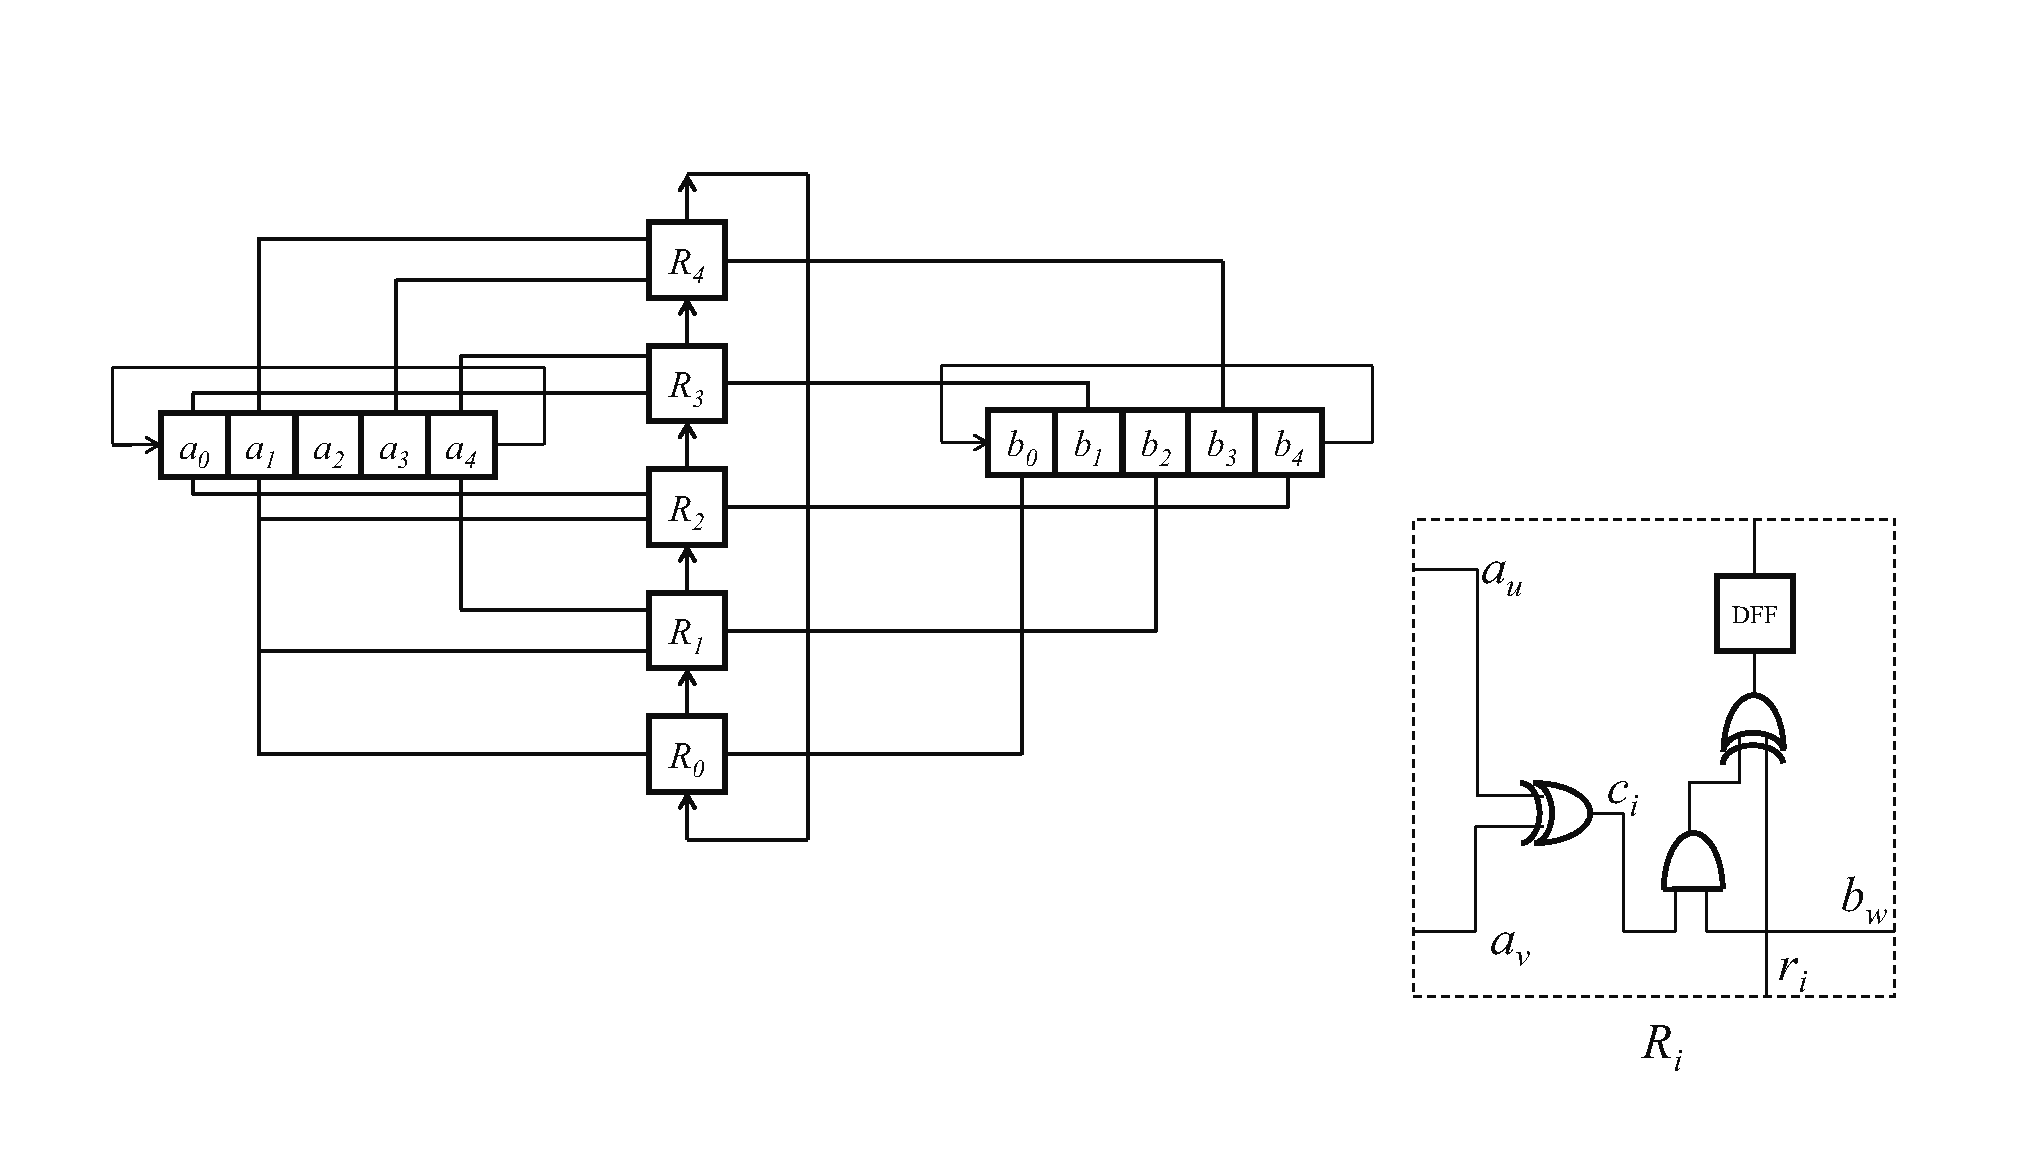
\includegraphics[width=\textwidth]{newfig/mySMPO.eps}
\caption{5-bit Agnew's SMPO. Index $i$ satisfies $0<i<4$, indices $u,v$ are determined by column \# of nonzero entries in $i$-th row of $\lambda$-Matrix $M^{(0)}$, i.e. if entry $M_{ij}^{(0)}$ is a nonzero entry, $u$ or $v$ equals to $i+j \pmod 5$. Index $w = 2i\pmod 5$}
\label{fig:SMPO}}
\end{figure}

\begin{Example}[5-bit Agnew's SMPO]
Given GF $\mathbb F_{2^5}$ and primitive element $\alpha$ defined by irreducible polynomial 
$\alpha^5+\alpha^2+1=0$, normal element $\beta = \alpha^5$ constructs an ONB $\{\beta,\beta^2,\beta^4,\beta^8,\beta^{16}\}$.
The $0$-th $\lambda$-Matrix for this ONB is
\begin{equation*}
M^{(0)} = \left(\begin{array}{lcccr}
0 &1 &0 &0 &0 \\
1 &0 &0 &1 &0 \\
0 &0 &0 &1 &1 \\
0 &1 &1 &0 &0 \\
0 &0 &1 &0 &1
\end{array}\right)
\end{equation*}
Then a typical design of 5-bit Agnew's SMPO is depicted in figure \ref{fig:SMPO}.

The operands part of this circuit is the same with Massey-Omura multiplier. The differences are on 
the matrix multiplication part, while it is implemented as separate logic blocks for 5 outputs,
and the 5 blocks are connected in a shift register fashion. By analyzing the detailed function of 
logic blocks, we can reveal the mechanism of Agnew's SMPO.

Suppose we implement $M^{(0)}$ as the logic block in SMSO. In the first clock cycle, the output is
\begin{equation}
\label{eqn:5bitSMPO_c0}
c_0 = a_1b_0+(a_0+a_3)b_1 + (a_3+a_4)b_2 + (a_1+a_2)b_3 + (a_2+a_4)b_4
\end{equation}
Note it is written in the form of equation \ref{eqn:SMPOterms}. In next clock cycles we can obtain 
remaining bits of the product, which can be written in following general form polynomial:
\begin{align}
c_i =& b_ia_{i+1} + b_{i+1}(a_i + a_{i+3}) + b_{i+2}(a_{i+3} + a_{i+4}) \nonumber\\
&+ b_{i+3}(a_{i+1} + a_{i+2}) + b_{i+4}
(a_{i+2} + a_{i+4}),\ 0\leq i\leq 4 \nonumber
\end{align}
Note all index calculations are reduced modulo 5.

Now let us observe the behavior of 5-bit Agnew's SMPO. Initially all DFFs are reset to 0. 
In the first clock cycle,
signal sent to the flip-flop in block $R_0$ denotes function:
$$R_0^{(1)} = a_1b_0$$
It equals to the first term of equation \ref{eqn:5bitSMPO_c0}. In the second clock cycle,
this signal is sent to block $R_1$ through wire $r_0$, and this block also receives data 
from operands (shifted by 1 bit), generating signal $a_u,a_v$ and $b_w$. Concretely,
signal sent to flip-flop in block $R_1$ is:
$$R_1^{(2)} = R_0^{(1)} + (a_0+a_3)b_1 = a_1b_0+(a_0+a_3)b_1$$
which forms first 2 terms of equation \ref{eqn:5bitSMPO_c0}. Similarly, we track the signal 
on $R_2$ in third clock cycle, signal on $R_3$ in fourth clock cycle, finally we can get 
$$R_4^{(5)} = a_1b_0+(a_0+a_3)b_1 + (a_3+a_4)b_2 + (a_1+a_2)b_3 + (a_2+a_4)b_4$$
which equals to $c_0$ in equation \ref{eqn:5bitSMPO_c0}.
After the fifth clock cycle ends, this signal can be detected on wire $r_0$. It shows that 
the result of $c_0$ is computed after 5 clock cycles and given on $r_0$.

If we track $R_1\to R_2\to R_3 \to \cdots \to R_0$, we can obtain $c_1$ respectively.
Thus we conclude that Agnew's SMPO functions the same with Massey-Omura multiplier.
\end{Example}

The design of Agnew's SMPO guarantees that there is only one AND gate in each $R_i$ block.
For ONB, adopting Agnew's SMPO will reduce the number of AND gates from $2k-1$ to $k$.

\subsection{Multiplier not based on $\lambda$-Matrix}
Both Massey-Omura multiplier and Agnew's SMPO rely on the implementation of $\lambda$-Matrix,
which means that they will be identical if unrolled to full combinational circuits. 
After Agnew's work of parallelization, researchers proposed more designs of SMPO, 
some of them jump out of the circle and are independent from $\lambda$-Matrix.
One competitive multiplier design of this type is invented by Reyhani-Masoleh and Hasan 
\cite{RHmulti}, which is therefore called RH-SMPO.

% fig:5bitRH

Figure \ref{fig:5bitRH} is a 5-bit RH-SMPO which is functionally equivalent to 5-bit Agnew's SMPO 
in figure \ref{fig:SMPO}. A brief proof is as follows: 

\begin{Proof}
First, we define an auxiliary function for $i$-th bit 
\begin{equation}
\label{eqn:aux}
F_i(A,B) = a_ib_i\beta + \sum_{j=1}^v d_{i,j}\beta^{1+2^j}
\end{equation}
where $0\leq i\leq k-1, v = \lfloor k/2\rfloor, 1\leq j \leq v$.
The $d$-layer index $d_{i,j}$ is defined as
\begin{equation}
\label{eqn:auxDC}
d_{i,j} = c_{a,i} c_{b,i} = (a_i+a_{i+j})(b_i+b_{i+j}),~~1\leq j\leq v
\end{equation}
$i+j$ here is the result reduced modulo $k$. Note that there is a special boundary case when
$k$ is an even number ($v = \frac{k}{2}$):
$$d_{i,v} = (a_i+a_{i+v})b_i$$
With the auxiliary function, we can utilize following theorem (proof refers to \cite{RHmulti}):
\begin{Theorem}
Consider three elements $A,B$ and $R$ such that $R=A\times B$ over $\Fkk$. Then,
$$R=(((F_{k-1}^2+F_{k-2})^2+F_{k-3})^2+\cdots+F_1)^2+F_0$$
\end{Theorem}
This form is called inductive sum of squares, and corresponds to the cyclic shifting on 
$R_i$ flip-flops. Concretely, the multiplier behavior is an implementation of 
following algorithm:

\begin{algorithm}[H]
\SetAlgoNoLine

 \KwIn{$A,B\in \Fkk$ given w.r.t. NB $N$}
 \KwOut{$R=A\times B$}
%%%%%%%%%%%%%%%%%%%%
  Initialize $A,B$ and aux var $X$ to 0\;
  \For { ($i=0$;   $i < k$; ++i ) }
  {
	$X \gets X^2+F_{k-1}(A,B)$ \CommentSty{/*use aux-func from Eq.\ref{eqn:aux}*/\;}
	$A\gets A^2,~B\gets B^2$ \CommentSty{/*Right-cyclic shift $A$ and $B$*/\;}
  }
  $R\gets X$
\caption{NB Multiplication Algorithm in RH-SMPO \cite{RHmulti}}\label{alg:RHmulti}
\end{algorithm}

In this algorithm, we use a fixed auxiliary function $F_{k-1}$ inside the loop.
This is because of equation
$$F_{k-l} = F_{k-1}(A^{2^{l-1}},B^{2^{l-1}}),~~1\le l\le k$$
So using fixed $F_{k-1}$ and squaring $A^{2^i}$ every time inside the loop is equivalent to computing 
$F_{k-1},F_{k-2},\dots,F_0$ with fixed operands $A,B$.
\end{Proof}

To better understand the mechanism of RH-SMPO, we will use this 5-bit 
RH-SMPO as an example and introduce the details on how to design it.
\begin{Example}[Designing a 5-bit RH-SMPO]
From equation \ref{eqn:aux} we can deploy AND gates in $d$-layer according to $d_{i,j}$,
and XOR gates in $c$-layer according to equation \ref{eqn:auxDC}. Concretely, as algorithm \ref{alg:RHmulti}
describes, we implement auxiliary function $F_{k-1}$ in the logic:
$$i = k-1 = 4;~~v=\lfloor 5/2 \rfloor = 2$$
\begin{equation}
\label{eqn:5bitRHaux}
F_{4}(A,B) = a_4b_4\beta+\sum_{j=1}^2 d_{4,j}\beta^{1+2^j} = d_0\beta+\sum_{j=1}^2 d_{4,j}\beta^{1+2^j}
\end{equation}
Consider indices $4+1=0\bmod 5,~4+2=1\bmod 5$, write down gates in $c$-layer and $d$-layer (besides $d_0$)
$$c_1 = a_0+a_4,~c_2 = b_0+b_4,~d_1=d_{4,1}= c_1c_2 = (a_4+a_0)(b_4+b_0)$$
$$c_3 = a_1+a_4,~c_4 = b_1+b_4,~d_2=d_{4,2}= c_3c_4 = (a_4+a_1)(b_4+b_1)$$
The difficult part of the whole design is to deploy XOR gates in $e$-layer. 
As the logic layer closest to the outputs $R_i$, $e$-layer actually finishes the implementation of 
$F_{k-1}(A,B)$. But it is not a simple addition; the reason is before bit-wise adding to $X^2$, it is necessary to 
turn the sum to NB form. In other words, theoretically we need $k$ XOR gates in $e$-layer, the output of 
$i$-th gate corresponds to the bit multiplying $\beta^{2^i}$.

In order to obtain information 
indicating interconnections between $d$-layer and $e$-layer, we need to interpret $\beta^{1+2^j}$ 
to NB representation.
There is a concept called {\bf multiplication table} (M-table) which can assist this interpretation. It is defined as 
a $k\times k$ matrix $T$ over $\mathbb F_2$:
\begin{equation}
\label{eqn:multitable}
\begin{bmatrix}
\beta^{1+2^0} \\ \beta^{1+2^1} \\ \beta^{1+2^2} \\ \vdots \\ \beta^{1+2^{k-1}}
\end{bmatrix}
= \beta
\begin{bmatrix}
\beta \\ \beta^2 \\ \beta^4 \\ \vdots \\ \beta^{2^{k-1}}
\end{bmatrix}
=
\begin{bmatrix}
T_{0,0}      &   T_{0,1}        & \dots & T_{0,k-1}\\
T_{1,0}    &   T_{1,1}           & \dots & T_{1,k-1}\\
T_{2,0}    &   T_{2,1}           & \dots & T_{2,k-1}\\
\vdots & \vdots              & \ddots     & \vdots \\
T_{k-1,0}    &   T_{k-1,1}           & \dots & T_{k-1,k-1}
\end{bmatrix}
\begin{bmatrix}
\beta \\ \beta^2 \\ \beta^4 \\ \vdots \\ \beta^{2^{k-1}}
\end{bmatrix}
= {\bf T}
\begin{bmatrix}
\beta \\ \beta^2 \\ \beta^4 \\ \vdots \\ \beta^{2^{k-1}}
\end{bmatrix}
\end{equation}

It is a known fact that M-table $T$ can be converted from $\lambda$-Matrix $M$:
$$M_{i,j}^{(0)} = T_{j-i,-i}$$
with indices reduced modulo $k$ (proof refers to appendix \ref{append:ONB}). Thus we can write down the M-table of $\mathbb F_{2^5}$ with current NB $N$:

% fig:multitable

Note that we only use row 1 and row 2 from the M-table since range $1\leq j \leq 2$.
All nonzero entries in these 2 rows corresponds to the interconnections between $d$-layer and 
$e$-layer. For example, row 1 has two nonzero entries at column 0 and column 3, which corresponds to interconnections 
between $d_1$ and $e_0,e_3$. This conclusion comes from row 1 in equation \ref{eqn:multitable}:
\begin{equation*}
\beta\cdot\beta^2 = 
\begin{bmatrix}
1 & 0 & 0 & 1 & 0
\end{bmatrix}
\begin{bmatrix}
\beta \\ \beta^2 \\ \beta^4 \\ \beta^8 \\ \beta^{16}
\end{bmatrix}
= \beta + \beta^{2^3}
\end{equation*}

Similarly, from row 2 of M-table we derive that $d_2$ has fanouts $e_3,e_4$:
\begin{equation*}
\beta\cdot\beta^{2^2} = 
\begin{bmatrix}
0 & 0 & 0 & 1 & 1
\end{bmatrix}
\begin{bmatrix}
\beta \\ \beta^2 \\ \beta^4 \\ \beta^8 \\ \beta^{16}
\end{bmatrix}
= \beta^{2^3} + \beta^{2^4}
\end{equation*}

Let us look back at equation \ref{eqn:5bitRHaux}, we already dealt with the latter part.
The first term is always $d_0\beta$, which denotes $d_0$ should always be connected to $e_0(\beta)$.
After gathering all interconnection information, we can translate it to gate-level circuit implementation:
$$e_0 = d_0+d_1,~e_3=d_1+d_2,~e_4=d_2$$

Then the last mission is to implement the output $R_i$ layer. Assume $r_{i-1}$ is the output of 
$R_{i-1}$ in last clock cycle, we can connect using relation 
$$R_i = r_{i-1} + e_i$$
In this example, according to the M-table in figure \ref{fig:multitable}, columns $e_1,e_2$
have only zeros in its intersection with row $d_1,d_2$. Thus gates for $e_1,e_2$ can be omitted.

This finishes the full design procedure for a 5-bit RH-SMPO.
\end{Example}

The area cost of RH-SMPO is even smaller than Agnew's SMPO. XOR gates corresponds to all nonzero entries 
in M-table, which is with the same number of nonzero entries in $\lambda$-Matrix ($C_N$). The number of AND gates 
equals to $v$ plus 1 (for gate $d_0$). When using ONB ($C_N = 2k-1$), the total number of gates 
is $2k+\lfloor \frac{k}{2}\rfloor$.

\section{Full-Blown Verification Procedure for Normal Basis Multiplier Functional Correctness Checking}
Once a gate-level design of a NB multiplier is generated, it is ready to be verified using 
similar approach appear in section \ref{sec:recha_approach}. The following part borrows contents
from my own conference paper \cite{myDATE}.
\subsection{Implicit Unrolling based on Abstraction with ATO}
In preliminaries we talk about the abstraction basics. If we use elimination term order 
$intermediate~variables~>~R~>~A,B$, the function of the combinational logic component 
can be abstracted as 
$$R = \Func(A,B)$$
If we are verifying the functional correctness of a combinational NB multiplier (e.g. Mastrovito multiplier
or Montgomery multiplier), the function given by abstraction will be $R=AB$.
While in the sequential case, the function of combinational logic only fulfills a part of the multiplication,
such as $F_{k-1}$ in equation \ref{eqn:aux}. Nevertheless, the abstraction still provides a word-level 
representation which works definitely better on unrolling than bit-level expressions.
In other words, with the assistance of abstraction, we can execute implicit unrolling instead of 
explicit unrolling and avoid bit-blasting problem.

For 2-input sequential NB multipliers, abstraction is utilized to implement following algorithm:
%\vspace{-0.1in}
\IncMargin{1em}
\begin{algorithm}[hbt]
\SetAlgoNoLine
\LinesNumbered
 \KwIn{Circuit polynomial ideal $J$, vanishing ideal $J_0$, initial
   state ideal $R (=0), \mathcal{G}(A_{init}), \mathcal{H}(B_{init})$} 

  $from_0(R,A,B) = \langle R, \mathcal{G}(A_{init}), \mathcal{H}(B_{init})\rangle$\;
  $i = 0$\;
  \Repeat{$i == k$}
  {
  	$i \gets i + 1$\;
%	$to^i(R',A',B') \gets$  $GB( \langle J_{ckt}, J_0,
%    from^{i-1}(R,A,B)\rangle )$ with abstraction term order\;
	$G \gets$GB$( \langle J + J_0+ from_{i-1}(R,A,B) \rangle
    )$ with ATO\;
	$to_i(R',A',B')\gets G\cap \mathbb F_{2^k}[R',A',B',R,A,B]$\;
	$from_i \gets to_i(\{R,A,B\}\setminus \{R',A',B'\})$\;
  }
\Return{$from_k(R_{final})$}
\caption {Abstraction via implicit unrolling for Sequential GF circuit
  verification}
\label{alg:modified}
\end{algorithm}
\DecMargin{1em}
%\vspace{-0.1in}

\begin{figure}[H]
\centering{
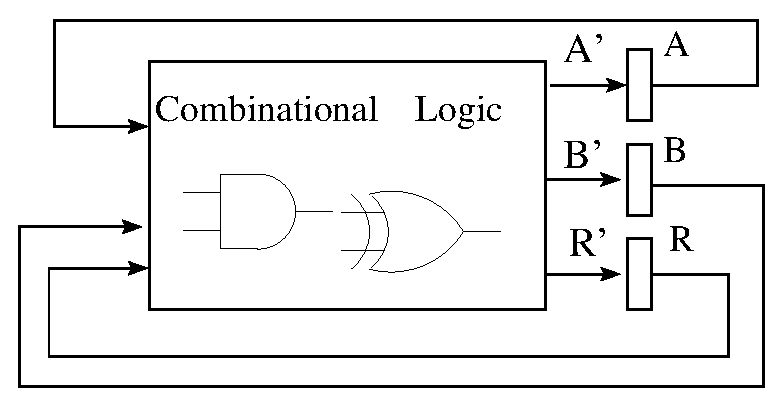
\includegraphics[width=5in]{newfig/gf_seq_model.eps}
\caption{A typical normal basis GF sequential circuit model. $A =
  (a_0,\dots,a_{k-1})$ and similarly $B, R$ are $k$-bit registers;
  $A', B', R'$ denote next-state inputs.}
\label{fig:sequential}}
\end{figure}

We follow  the sequential GF circuit model of
figure \ref{fig:sequential}, with word-level variables $A, B, R$
denoting {\it present states (PS)} and $A', B', R'$ denoting {\it next
  states (NS)} of the machine; where $A = \sum_{i=0}^{k-1} a_i \beta^{2^i}$
for the PS variables and $A' = \sum_{i=0}^{k-1} a_i'
\beta^{2^i}$ for NS variables, and so on.  Variables $R\ (R')$ correspond to those that 
store the result, and $A, B\ (A', B')$ store input operands. E.g.,
for a GF multiplier, $A_{init}, B_{init}$ (and $R_{init} =
0$) are the initial values (operands) loaded into the registers,  and
$R = \Func(A_{init}, B_{init}) = A_{init} \times B_{init}$ is the final
result after $k$-cycles. Our approach aims to find this polynomial
representation for $R$.  

Each gate in the combinational logic is represented by a Boolean
polynomial. To 
this set of Boolean polynomials, we append the polynomials that define
the word-level to bit-level relations for PS and NS variables ($A =
\sum_{i=0}^{k-1} a_i \beta^{2^i}$). We denote this set of polynomials
as ideal $J = \langle 
f_1, \dots, f_s \rangle \subset \Fkk[x_1, \dots, x_d, R, R', A, A', B,
  B']$, where $x_1, \dots, x_d$ denote the bit-level (Boolean) variables
  of the circuit. The ideal of vanishing polynomials $J_0$ is also included, and
then the implicit FSM unrolling problem is setup for abstraction. 

The configurations of the flip-flops are the states of the
machine. Since the set of states is a finite set of points, we
can consider it as the variety of an ideal related to the circuit.
Moreover, since we are interested in
the function encoded by the state variables (over $k$-time
frames), we can project this variety on the word-level state
variables, starting from the initial state $A_{init}, B_{init}$.
Projection of varieties (geometry) corresponds to elimination ideals
(algebra), and can be analyzed via \Grobner bases. Therefore, we
employ a \Grobner basis computation with ATO: we use a {\it lex term
  order} with {\it bit-level variables} 
$>$ {\it word-level NS outputs} $>$ {\it word-level PS inputs}. This
allows to eliminate all the bit-level variables 
%(corresponding to the combinational logic and the state variables),
%so as to 
and derives a representation only in terms of words. 
Consequently, $k$-successive \Grobner basis computations implicitly
unroll the machine, and provide word-level algebraic $k$-cycle
abstraction for $R'$ as $R' = \F(A_{init}, B_{init})$. 

Algorithm
\ref{alg:modified} describes our approach.  In the algorithm, $from_i$
and $to_i$ are polynomial ideals whose varieties are the valuations of
word-level variables $R, A, B$ and $R',A',B'$ in the $i$-th iteration;
and the notation ``$\setminus$'' signifies that the $NS$ in iteration
$(i)$ becomes the $PS$ in iteration $(i+1)$. Line 5 computes the Gr\"obner 
basis with the abstraction term order.  Line 6 computes the elimination 
ideal, eliminating the bit-level variables and representing the set of 
reachable states up to iteration $i$ in terms of the elimination ideal. 
These computations are analogous to those of image computations performed in FSM reachability. 
\begin{Example}[Functional verification of 5-bit RH-SMPO]
\label{ex:RHSMPO}
Figure \ref{fig:5bitRH} shows the detailed structure of a 5-bit RH-SMPO. The transition function for
operands $A,B$ is doing cyclic shift, while transition function for $R$ has to be computed through Gr\"obner basis
abstraction approach. Following ideal $J_{ckt}$ from line 5 in algorithm \ref{alg:modified} is the ideal for 
all gates in combinational logic block and definition of word-level variables.
\begin{align}
J_{ckt} = & d_0+a_4b_4, c_1+a_0+a_4, c_2+b_0+b_4, d_1+c_1c_2, c_3+a_1a_4,\nonumber\\
& c_4+b_1b_4, d_2+c_3c_4, e_0+d_0+d_1, e_3+d_1+d_2, e_4+d_2, \nonumber\\
& R_0+r_4+e_0, R_1+r_0, R_2+r_1, R_3+r_2+e_3, R_4+r_3+e_4,\nonumber\\
& A+a_0\alpha^5+a_1\alpha^{10}+a_2\alpha^{20}+a_3\alpha^9+a_4\alpha^{18},\nonumber\\
		 & B+b_0\alpha^5+b_1\alpha^{10}+b_2\alpha^{20}+b_3\alpha^9+b_4\alpha^{18},\nonumber\\
		 & R'+r_0'\alpha^5+r_1'\alpha^{10}+r_2'\alpha^{20}+r_3'\alpha^9+r_4'\alpha^{18},\nonumber\\
		 & R+R_0\alpha^5+R_1\alpha^{10}+R_2\alpha^{20}+R_3\alpha^9+R_4\alpha^{18};\nonumber
\end{align}
In our implementation here, since we only focus on the output variable $R$, evaluations of intermediate input 
operands $A, B$ are unnecessary. Polynomials about $A$ and $B$ can be removed from $J_{ckt}$, and $R$ is directly
evaluated by initial operands $A_{init}$ and $B_{init}$, which are associated with present state bit-level inputs
$a_0,a_1,\dots,a_4$ and $b_0,b_1,\dots,b_4$ by polynomials in $from^i$.

According to line 5 of algorithm \ref{alg:modified}, we merge $J_{ckt}$, $J_0$ and $from^i$, then compute its
Gr\"obner basis with abstraction term order (copy details here). There is a polynomial in form of $R'+\Func(A_{init},B_{init})$,
which should be included by $to^{i+1}$. $to^{i+1}$ also exclude next state variable $A'$ and $B'$, instead we 
redefine $A_{init}$ and $B_{init}$ using next state bit-level variables $\{a_i', b_j'\}$. Next state Bit-level variables
$a_i' = a_{i-1\pmod k}, b_j' = b_{j-1\pmod k}$ according to definition of cyclic shift.

Line 7 in algorithm \ref{alg:modified} is implemented by replacing $R'$ with $R$, $\{a_i', b_j'\}$ with $\{a_i,b_j\}$.

All intermediate results for each clock cycle are listed below:
\begin{itemize}
\item Clock 1: ${\bf from^0} = \{R, A_{init}+a_0\alpha^5+a_1\alpha^{10}+a_2\alpha^{20}+a_3\alpha^9+a_4\alpha^{18},
B_{init}+b_0\alpha^5+b_1\alpha^{10}+b_2\alpha^{20}+b_3\alpha^9+b_4\alpha^{18}\}$, \\
	${\bf to^1} = \{R'+(\alpha^4+\alpha^3+1) A_{init}^{16} B_{init}^{16}+(\alpha^4+\alpha^2) A_{init}^{16} B_{init}^4+(\alpha^3+1) A_{init}^{16} B_{init}^2+(\alpha^4+\alpha^3+1) A_{init}^{16} B_{init}+(\alpha^4+\alpha^3+\alpha^2+1) A_{init}^8 B_{init}^8+(\alpha^4+\alpha^3+\alpha+1) A_{init}^8 B_{init}^4+(\alpha^3+\alpha+1) A_{init}^8 B_{init}^2+(\alpha^4+\alpha^2) A_{init}^8 B_{init}+(\alpha^4+\alpha^2) A_{init}^4 B_{init}^{16}+(\alpha^4+\alpha^3+\alpha+1) A_{init}^4 B_{init}^8+(\alpha^2) A_{init}^4 B_{init}^4+(\alpha^3+\alpha^2+\alpha+1) A_{init}^4 B_{init}^2+(\alpha^4+\alpha^3+\alpha+1) A_{init}^4 B_{init}+(\alpha^3+1) A_{init}^2 B_{init}^{16}+(\alpha^3+\alpha+1) A_{init}^2 B_{init}^8+(\alpha^3+\alpha^2+\alpha+1) A_{init}^2 B_{init}^4+(\alpha^3+\alpha^2+\alpha) A_{init}^2 B_{init}^2+(\alpha^4+\alpha) A_{init}^2 B_{init}+(\alpha^4+\alpha^3+1) A_{init} B_{init}^{16}+(\alpha^4+\alpha^2) A_{init} B_{init}^8+(\alpha^4+\alpha^3+\alpha+1) A_{init} B_{init}^4+(\alpha^4+\alpha) A_{init} B_{init}^2+(\alpha^3+\alpha+1) A_{init} B_{init},
	A_{init}+a_4'\alpha^5+a_0'\alpha^{10}+a_1'\alpha^{20}+a_2'\alpha^9+a_3'\alpha^{18},
B_{init}+b_4'\alpha^5+b_0'\alpha^{10}+b_1'\alpha^{20}+b_2'\alpha^9+b_3'\alpha^{18}\}$
\item Clock 2: ${\bf from^1} = \{R+(\alpha^4+\alpha^3+1) A_{init}^{16} B_{init}^{16}+(\alpha^4+\alpha^2) A_{init}^{16} B_{init}^4+(\alpha^3+1) A_{init}^{16} B_{init}^2+(\alpha^4+\alpha^3+1) A_{init}^{16} B_{init}+(\alpha^4+\alpha^3+\alpha^2+1) A_{init}^8 B_{init}^8+(\alpha^4+\alpha^3+\alpha+1) A_{init}^8 B_{init}^4+(\alpha^3+\alpha+1) A_{init}^8 B_{init}^2+(\alpha^4+\alpha^2) A_{init}^8 B_{init}+(\alpha^4+\alpha^2) A_{init}^4 B_{init}^{16}+(\alpha^4+\alpha^3+\alpha+1) A_{init}^4 B_{init}^8+(\alpha^2) A_{init}^4 B_{init}^4+(\alpha^3+\alpha^2+\alpha+1) A_{init}^4 B_{init}^2+(\alpha^4+\alpha^3+\alpha+1) A_{init}^4 B_{init}+(\alpha^3+1) A_{init}^2 B_{init}^{16}+(\alpha^3+\alpha+1) A_{init}^2 B_{init}^8+(\alpha^3+\alpha^2+\alpha+1) A_{init}^2 B_{init}^4+(\alpha^3+\alpha^2+\alpha) A_{init}^2 B_{init}^2+(\alpha^4+\alpha) A_{init}^2 B_{init}+(\alpha^4+\alpha^3+1) A_{init} B_{init}^{16}+(\alpha^4+\alpha^2) A_{init} B_{init}^8+(\alpha^4+\alpha^3+\alpha+1) A_{init} B_{init}^4+(\alpha^4+\alpha) A_{init} B_{init}^2+(\alpha^3+\alpha+1) A_{init} B_{init},
	A_{init}+a_4\alpha^5+a_0\alpha^{10}+a_1\alpha^{20}+a_2\alpha^9+a_3\alpha^{18},
B_{init}+b_4\alpha^5+b_0\alpha^{10}+b_1\alpha^{20}+b_2\alpha^9+b_3\alpha^{18}\}$, \\
${\bf to^2} = \{R'+(\alpha^3+\alpha+1) A_{init}^{16} B_{init}^{16}+(\alpha^4+\alpha^3+1) A_{init}^{16} B_{init}^8+(\alpha^2) A_{init}^{16} B_{init}^4+(\alpha^3+1) A_{init}^{16} B_{init}^2+(\alpha^4+\alpha^3+1) A_{init}^8 B_{init}^{16}+(\alpha^4+\alpha^2) A_{init}^8 B_{init}^8+(\alpha^4) A_{init}^8 B_{init}^4+(\alpha^4+\alpha^3+1) A_{init}^8 B_{init}^2+(\alpha^3+1) A_{init}^8 B_{init}+(\alpha^2) A_{init}^4 B_{init}^{16}+(\alpha^4) A_{init}^4 B_{init}^8+(\alpha^4) A_{init}^4 B_{init}^4+(\alpha^4+\alpha^3+\alpha+1) A_{init}^4 B_{init}^2+(\alpha) A_{init}^4 B_{init}+(\alpha^3+1) A_{init}^2 B_{init}^{16}+(\alpha^4+\alpha^3+1) A_{init}^2 B_{init}^8+(\alpha^4+\alpha^3+\alpha+1) A_{init}^2 B_{init}^4+(\alpha^2) A_{init}^2 B_{init}^2+(\alpha^4+\alpha^3+\alpha^2+\alpha+1) A_{init}^2 B_{init}+(\alpha^3+1) A_{init} B_{init}^8+(\alpha) A_{init} B_{init}^4+(\alpha^4+\alpha^3+\alpha^2+\alpha+1) A_{init} B_{init}^2+(\alpha^4+\alpha^3+\alpha^2+\alpha+1) A_{init} B_{init},
A_{init}+a_3'\alpha^5+a_4'\alpha^{10}+a_0'\alpha^{20}+a_1'\alpha^9+a_2'\alpha^{18},
B_{init}+b_3'\alpha^5+b_4'\alpha^{10}+b_0'\alpha^{20}+b_1'\alpha^9+b_2'\alpha^{18}\}$
\item Clock 3: ${\bf from^2} = \{R+(\alpha^3+\alpha+1) A_{init}^{16} B_{init}^{16}+(\alpha^4+\alpha^3+1) A_{init}^{16} B_{init}^8+(\alpha^2) A_{init}^{16} B_{init}^4+(\alpha^3+1) A_{init}^{16} B_{init}^2+(\alpha^4+\alpha^3+1) A_{init}^8 B_{init}^{16}+(\alpha^4+\alpha^2) A_{init}^8 B_{init}^8+(\alpha^4) A_{init}^8 B_{init}^4+(\alpha^4+\alpha^3+1) A_{init}^8 B_{init}^2+(\alpha^3+1) A_{init}^8 B_{init}+(\alpha^2) A_{init}^4 B_{init}^{16}+(\alpha^4) A_{init}^4 B_{init}^8+(\alpha^4) A_{init}^4 B_{init}^4+(\alpha^4+\alpha^3+\alpha+1) A_{init}^4 B_{init}^2+(\alpha) A_{init}^4 B_{init}+(\alpha^3+1) A_{init}^2 B_{init}^{16}+(\alpha^4+\alpha^3+1) A_{init}^2 B_{init}^8+(\alpha^4+\alpha^3+\alpha+1) A_{init}^2 B_{init}^4+(\alpha^2) A_{init}^2 B_{init}^2+(\alpha^4+\alpha^3+\alpha^2+\alpha+1) A_{init}^2 B_{init}+(\alpha^3+1) A_{init} B_{init}^8+(\alpha) A_{init} B_{init}^4+(\alpha^4+\alpha^3+\alpha^2+\alpha+1) A_{init} B_{init}^2+(\alpha^4+\alpha^3+\alpha^2+\alpha+1) A_{init} B_{init},
A_{init}+a_3\alpha^5+a_4\alpha^{10}+a_0\alpha^{20}+a_1\alpha^9+a_2\alpha^{18},
B_{init}+b_3\alpha^5+b_4\alpha^{10}+b_0\alpha^{20}+b_1\alpha^9+b_2\alpha^{18}\}$, \\
${\bf to^3} = \{R'+(\alpha^4+\alpha^3+1) A_{init}^{16} B_{init}^{16}+(\alpha) A_{init}^{16} B_{init}^8+(\alpha^4+\alpha^3+\alpha^2+1) A_{init}^{16} B_{init}^4+(\alpha^4+\alpha^3+\alpha^2+\alpha+1) A_{init}^{16} B_{init}^2+(\alpha^4+\alpha^3+\alpha^2+1) A_{init}^{16} B_{init}+(\alpha) A_{init}^8 B_{init}^{16}+(\alpha+1) A_{init}^8 B_{init}^8+(\alpha^4) A_{init}^8 B_{init}^4+(\alpha^3+\alpha^2+1) A_{init}^8 B_{init}^2+(\alpha^4+\alpha^3+\alpha+1) A_{init}^8 B_{init}+(\alpha^4+\alpha^3+\alpha^2+1) A_{init}^4 B_{init}^{16}+(\alpha^4) A_{init}^4 B_{init}^8+(\alpha^4+\alpha^3+\alpha+1) A_{init}^4 B_{init}^4+(\alpha^3+\alpha+1) A_{init}^4 B_{init}^2+(\alpha^4+\alpha^3+\alpha^2+\alpha+1) A_{init}^4 B_{init}+(\alpha^4+\alpha^3+\alpha^2+\alpha+1) A_{init}^2 B_{init}^{16}+(\alpha^3+\alpha^2+1) A_{init}^2 B_{init}^8+(\alpha^3+\alpha+1) A_{init}^2 B_{init}^4+(\alpha^3+\alpha+1) A_{init}^2 B_{init}^2+(\alpha^4+\alpha^3+\alpha^2+1) A_{init} B_{init}^{16}+(\alpha^4+\alpha^3+\alpha+1) A_{init} B_{init}^8+(\alpha^4+\alpha^3+\alpha^2+\alpha+1) A_{init} B_{init}^4+(\alpha^4+\alpha) A_{init} B_{init},
A_{init}+a_2'\alpha^5+a_3'\alpha^{10}+a_4'\alpha^{20}+a_0'\alpha^9+a_1'\alpha^{18},
B_{init}+b_2'\alpha^5+b_3'\alpha^{10}+b_4'\alpha^{20}+b_0'\alpha^9+b_1'\alpha^{18}\}$
\item Clock 4: ${\bf from^3} = \{R+(\alpha^4+\alpha^3+1) A_{init}^{16} B_{init}^{16}+(\alpha) A_{init}^{16} B_{init}^8+(\alpha^4+\alpha^3+\alpha^2+1) A_{init}^{16} B_{init}^4+(\alpha^4+\alpha^3+\alpha^2+\alpha+1) A_{init}^{16} B_{init}^2+(\alpha^4+\alpha^3+\alpha^2+1) A_{init}^{16} B_{init}+(\alpha) A_{init}^8 B_{init}^{16}+(\alpha+1) A_{init}^8 B_{init}^8+(\alpha^4) A_{init}^8 B_{init}^4+(\alpha^3+\alpha^2+1) A_{init}^8 B_{init}^2+(\alpha^4+\alpha^3+\alpha+1) A_{init}^8 B_{init}+(\alpha^4+\alpha^3+\alpha^2+1) A_{init}^4 B_{init}^{16}+(\alpha^4) A_{init}^4 B_{init}^8+(\alpha^4+\alpha^3+\alpha+1) A_{init}^4 B_{init}^4+(\alpha^3+\alpha+1) A_{init}^4 B_{init}^2+(\alpha^4+\alpha^3+\alpha^2+\alpha+1) A_{init}^4 B_{init}+(\alpha^4+\alpha^3+\alpha^2+\alpha+1) A_{init}^2 B_{init}^{16}+(\alpha^3+\alpha^2+1) A_{init}^2 B_{init}^8+(\alpha^3+\alpha+1) A_{init}^2 B_{init}^4+(\alpha^3+\alpha+1) A_{init}^2 B_{init}^2+(\alpha^4+\alpha^3+\alpha^2+1) A_{init} B_{init}^{16}+(\alpha^4+\alpha^3+\alpha+1) A_{init} B_{init}^8+(\alpha^4+\alpha^3+\alpha^2+\alpha+1) A_{init} B_{init}^4+(\alpha^4+\alpha) A_{init} B_{init},
A_{init}+a_2\alpha^5+a_3\alpha^{10}+a_4\alpha^{20}+a_0\alpha^9+a_1\alpha^{18},
B_{init}+b_2\alpha^5+b_3\alpha^{10}+b_4\alpha^{20}+b_0\alpha^9+b_1\alpha^{18}\}$, \\
${\bf to^4} = \{R'+(\alpha^3+\alpha+1) A_{init}^{16} B_{init}^{16}+(\alpha^4+\alpha^3+\alpha^2+\alpha+1) A_{init}^{16} B_{init}^8+(\alpha^4+\alpha) A_{init}^{16} B_{init}^4+(\alpha^3+1) A_{init}^{16} B_{init}^2+(\alpha^3+\alpha+1) A_{init}^{16} B_{init}+(\alpha^4+\alpha^3+\alpha^2+\alpha+1) A_{init}^8 B_{init}^{16}+(\alpha^3+1) A_{init}^8 B_{init}^8+(\alpha^4+\alpha^2+\alpha) A_{init}^8 B_{init}^4+(\alpha^2+\alpha) A_{init}^8 B_{init}^2+(\alpha^3+\alpha^2+1) A_{init}^8 B_{init}+(\alpha^4+\alpha) A_{init}^4 B_{init}^{16}+(\alpha^4+\alpha^2+\alpha) A_{init}^4 B_{init}^8+(\alpha^4+\alpha^2+\alpha) A_{init}^4 B_{init}^4+(\alpha^2+\alpha) A_{init}^4 B_{init}+(\alpha^3+1) A_{init}^2 B_{init}^{16}+(\alpha^2+\alpha) A_{init}^2 B_{init}^8+(\alpha^4+\alpha^2) A_{init}^2 B_{init}^2+(\alpha^3+\alpha^2+1) A_{init}^2 B_{init}+(\alpha^3+\alpha+1) A_{init} B_{init}^{16}+(\alpha^3+\alpha^2+1) A_{init} B_{init}^8+(\alpha^2+\alpha) A_{init} B_{init}^4+(\alpha^3+\alpha^2+1) A_{init} B_{init}^2+(\alpha) A_{init} B_{init},
A_{init}+a_1'\alpha^5+a_2'\alpha^{10}+a_3'\alpha^{20}+a_4'\alpha^9+a_0'\alpha^{18},
B_{init}+b_1'\alpha^5+b_2'\alpha^{10}+b_3'\alpha^{20}+b_4'\alpha^9+b_0'\alpha^{18}\}$
\item Clock 5: ${\bf from^4} = \{R+(\alpha^3+\alpha+1) A_{init}^{16} B_{init}^{16}+(\alpha^4+\alpha^3+\alpha^2+\alpha+1) A_{init}^{16} B_{init}^8+(\alpha^4+\alpha) A_{init}^{16} B_{init}^4+(\alpha^3+1) A_{init}^{16} B_{init}^2+(\alpha^3+\alpha+1) A_{init}^{16} B_{init}+(\alpha^4+\alpha^3+\alpha^2+\alpha+1) A_{init}^8 B_{init}^{16}+(\alpha^3+1) A_{init}^8 B_{init}^8+(\alpha^4+\alpha^2+\alpha) A_{init}^8 B_{init}^4+(\alpha^2+\alpha) A_{init}^8 B_{init}^2+(\alpha^3+\alpha^2+1) A_{init}^8 B_{init}+(\alpha^4+\alpha) A_{init}^4 B_{init}^{16}+(\alpha^4+\alpha^2+\alpha) A_{init}^4 B_{init}^8+(\alpha^4+\alpha^2+\alpha) A_{init}^4 B_{init}^4+(\alpha^2+\alpha) A_{init}^4 B_{init}+(\alpha^3+1) A_{init}^2 B_{init}^{16}+(\alpha^2+\alpha) A_{init}^2 B_{init}^8+(\alpha^4+\alpha^2) A_{init}^2 B_{init}^2+(\alpha^3+\alpha^2+1) A_{init}^2 B_{init}+(\alpha^3+\alpha+1) A_{init} B_{init}^{16}+(\alpha^3+\alpha^2+1) A_{init} B_{init}^8+(\alpha^2+\alpha) A_{init} B_{init}^4+(\alpha^3+\alpha^2+1) A_{init} B_{init}^2+(\alpha) A_{init} B_{init},
A_{init}+a_1\alpha^5+a_2\alpha^{10}+a_3\alpha^{20}+a_4\alpha^9+a_0\alpha^{18},
B_{init}+b_1\alpha^5+b_2\alpha^{10}+b_3\alpha^{20}+b_4\alpha^9+b_0\alpha^{18}\}$, \\
${\bf to^5} = \{{\bf R'+A_{init}B_{init}},
A_{init}+a_0'\alpha^5+a_1'\alpha^{10}+a_2'\alpha^{20}+a_3'\alpha^9+a_4'\alpha^{18},
B_{init}+b_0'\alpha^5+b_1'\alpha^{10}+b_2'\alpha^{20}+b_3'\alpha^9+b_4'\alpha^{18}\}$
\end{itemize}
The final result is
$from^5(R_{final}) = R_{final}+A_{init}\cdot B_{init}$
\end{Example}
\subsection{Overcome Computational Complexity using RATO}
Similar to our improvements in section \ref{sec:reachaRATO}, RATO \cite{TimDAC} is also available to 
accelerate the GB computation here. More specifically, we obviate GB computation by turning it 
into a single-step multivariate polynomial division: first, in ideal generated by
gates information polynomials and word-level variable definition polynomials, find the unique pair of polynomial
generators with leading monomials not relatively prime to each other; then, compute their specification polynomial
using definition 
$$Spoly(f_w,f_g) = \frac{LCM}{lt(f_w)}\cdot f_w - \frac{LCM}{lt(f_g)}\cdot f_g$$
where $LCM$ is least common multiple of $lm(f_w)$ and $lm(f_g)$, and $lt$ denotes the leading term;
last, reduce $Spoly$ with ideal $J_{ckt}+J_0$, it is possible that the remainder will be canonical polynomial
function of the circuit. We will illustrate the whole improved procedure by applying RATO on 
5-bit RH-SMPO in figure \ref{fig:5bitRH}.

\begin{Example}
\label{ex:newRATO}
Variable order under RATO is:
\begin{align}
&\{r_0',r_1',r_2',r_3',r_4'\}>\{r_0,r_1,r_2,r_3,r_4\}\nonumber\\
&>\{e_0,e_3,e_4\},\{d_0,d_1,d_2\},\{c_1,c_2,c_3,c_4\}\nonumber\\
&>\{a_0,a_1,a_2,a_3,a_4,b_0,b_1,b_2,b_3,b_4\}>R'>R>\{A,B\}\nonumber
\end{align}
Search among all generators of $J_{ckt}$ from Ex.\ref{ex:RHSMPO} using RATO, we find a pair of polynomials whose leading 
monomials are not relatively prime:
$(f_w,f_g), f_w = r_0'+r_4+e_0, f_g =r_0'\alpha^5+r_1'\alpha^{10}+r_2'\alpha^{20}+r_3'\alpha^9+r_4'\alpha^{18} + R'$.
We calculate $Spoly$ can reduce it by $J_{ckt}+J_0$:
\begin{align}
&Spoly(f_w,f_g) \xrightarrow{J_{ckt}+J_0}_{+}\nonumber\\
&(\alpha^3+\alpha^2+\alpha) r_1+(\alpha^4+\alpha^3+\alpha^2) r_2+(\alpha^2+\alpha) r_3+(\alpha) r_4\nonumber\\
&+(\alpha^3+\alpha^2) a_1 b_1+(\alpha^4+\alpha^3+\alpha^2+\alpha) a_1 b_2+(\alpha^2+\alpha) a_1 b_3\nonumber\\
&+(\alpha^2+1) a_1 b_4+(\alpha^4+1) a_1 B+(\alpha^4+\alpha) a_2 b_1+(\alpha^4+\alpha^3+\alpha) a_2 b_2\nonumber\\
&+(\alpha^3+1) a_2 b_3+(\alpha^3+\alpha^2+1) a_2 b_4+(\alpha^3+\alpha^2) a_2 B+(\alpha^2+\alpha) a_3 b_1\nonumber\\
&+(\alpha^3+1) a_3 b_2+(\alpha+1) a_3 b_3+(\alpha^4+\alpha^2+\alpha) a_3 b_4\nonumber\\
&+(\alpha^4+\alpha^3+\alpha) a_3 B+(\alpha^3+1) a_4 b_1+a_4 b_2+(\alpha^4+\alpha^2+\alpha) a_4 b_3\nonumber\\
&+(\alpha^4+\alpha^3+1) a_4 b_4+(\alpha^2+\alpha) a_4 B+(\alpha^4+1) b_1 A+(\alpha^3+\alpha^2) b_2 A\nonumber\\
&+(\alpha^4+\alpha^3+\alpha) b_3 A+(\alpha^2+\alpha) b_4 A+(\alpha^4+\alpha^2+\alpha+1) R'+R+A B\nonumber
\end{align}
\end{Example}
Above example indicates that RATO based abstraction on 5-bit RH-SMPO will result a remainder contains both
bit-level variables and word-level variables, and the number of remaining variables is still large such that
Gr\"obner basis computation will be inefficient.

Since the remainder from \emph{Spoly} reduction contains some bit-level variables, our objective is to compute
a polynomial contains only word-level variables (such as $R'+\mathcal{F}(A,B)$). One possible solution to
this problem is to replace bit-level variable monomials by equivalent polynomials that only contain word-level
variables, e.g. $a_i = \mathcal{G}(A), r_j = \mathcal{H}(R)$. In this section a Gaussian-elimination-fashion 
approach is introduced to compute corresponding $\mathcal{G}(A),\mathcal{H}(R)$ efficiently.

\begin{Example}
\label{ex:BLVS}
{\bf Objective}:\ Compute polynomial $a_i + \mathcal{G}_i(A)$ from $f_0 = a_0\alpha^5+a_1\alpha^{10}+a_2\alpha^{20}+a_3\alpha^9+a_4\alpha^{18}+A
 = g_0 + A$.

First, compute $f_0^2= a_0\alpha^{10}+a_1\alpha^{20}+a_2\alpha^{9}+a_3\alpha^{18}+a_4\alpha^{5}+A^2 = g_0^2 + A^2$;
then $f_0^4, f_0^8, f_0^{16}$. By repeating squaring we get a system of equations:
\begin{displaymath}
  \begin{cases}
  f_0  &=\ \  0\\
  f_0^2 & =\ \  0\\
  f_0^4  &=\ \  0\\
  f_0^8  &=\ \  0\\
  f_0^{16} & =\ \ 0
  \end{cases}
\Longleftrightarrow\ \
\begin{cases}
  g_0 & =\ \  A\\
  g_0^2 & =\ \  A^2\\
  g_0^4 & =\ \  A^4\\
  g_0^8 & =\ \  A^8\\
  g_0^{16} & =\ \  A^{16}
  \end{cases}
\end{displaymath}
Following is the coefficients matrix form of this system of equations:
\begin{displaymath}
\begin{pmatrix}
\alpha^5 & \alpha^{10} & \alpha^{20} & \alpha^9 & \alpha^{18} \\
\alpha^{10} & \alpha^{20} & \alpha^9 & \alpha^{18} & \alpha^5 \\
\alpha^{20} & \alpha^9 & \alpha^{18} & \alpha^5 & \alpha^{10} \\
\alpha^9 & \alpha^{18} & \alpha^5 & \alpha^{10} & \alpha^{20} \\
\alpha^{18} & \alpha^5 & \alpha^{10} & \alpha^{20} & \alpha^9 
\end{pmatrix}
\begin{pmatrix}
a_0\\
a_1\\
a_2\\
a_3\\
a_4
\end{pmatrix}
=
\begin{pmatrix}
A\\
A^2\\
A^4\\
A^8\\
A^{16}
\end{pmatrix}
\end{displaymath}

Use Gaussian elimination on coefficients matrix, for example  
\begin{align}
Row\ 2 =& Row\ 1\times \alpha^5 + Row\ 2: \nonumber\\
&a_1+(\alpha)a_2+(\alpha^4+\alpha^2)a_3+(\alpha^3+\alpha^2)a_4\nonumber\\
=&(\alpha^4+\alpha^3+\alpha^2+1)A^2+(\alpha^2+\alpha)A\nonumber
\end{align}
Recursively eliminate $a_1$ from third row, $a_2$ from fourth row, etc. The final solution to this system of
equations is
%\begin{displaymath}
%\{g_i\ | \ g_i: a_i + \mathcal{G}_i(A)\}
%\end{displaymath}
%\end{Example}
\begin{displaymath}
\left\{
  \begin{array}{lcl}
  a_0 & = & (\alpha+1)A^{16}+(\alpha^4+\alpha^3+\alpha)A^8+(\alpha^3+\alpha^2)A^4\\&&+(\alpha^4+1)A^2+(\alpha^2+1)A\\
  a_1 & = & (\alpha^2+1)A^{16}+(\alpha+1)A^8+(\alpha^4+\alpha^3+\alpha)A^4\\&&+(\alpha^3+\alpha^2)A^2+(\alpha^4+1)A\\
  a_2 & = & (\alpha^4+1)A^{16}+(\alpha^2+1)A^8+(\alpha+1)A^4\\&&+(\alpha^4+\alpha^3+\alpha)A^2+(\alpha^3+\alpha^2)A\\
  a_3 & = & (\alpha^3+\alpha^2)A^{16}+(\alpha^4+1)A^8+(\alpha^2+1)A^4\\&&+(\alpha+1)A^2+(\alpha^4+\alpha^3+\alpha)A\\
  a_4 & = & (\alpha^4+\alpha^3+\alpha)A^{16}+(\alpha^3+\alpha^2)A^8+(\alpha^4+1)A^4\\&&+(\alpha^2+1)A^2+(\alpha+1)A
  \end{array} \right.
\end{displaymath}
\end{Example}
Similarly we can compute equivalent polynomials $\mathcal{H}_i(R)$ for $r_i$, $\mathcal{T}_j(B)$ for $b_j$.
Using those polynomial equations, it is sufficient to translate all bit-level inputs in the remainder polynomial
because of following lemma:
\begin{Lemma}
\label{lem:bitlevelremainder}
Remainder of S-poly reduction will only contain primary inputs (bit-level) and word-level output; furthermore, there will be one and
only one term containing word-level output whose monomial is word-level output itself rather than higher order form.
\end{Lemma}

\begin{Proof}
First proposition is easy to prove by contradiction: assume there exists an intermediate bit-level variable $v$ in the remainder,
then this remainder must be divided further by a polynomial with leading term $v$. 
Since the remainder cannot be divided by any other polynomials in $J_{ckt}$, the assumption does not hold.

Second part, the candidate pair of polynomials only have one term of
single word-level output variable (say it is $R$) and this term is the last term under RATO, which means there is only one term with
$R$ in Spoly. Meanwhile in other polynomials from $J_{ckt}+J_0$ there is no such term containing $R$, so this term will be
kept to remainder $r$, with exponent equals to 1.
\end{Proof}

By replacing all bit-level variables by corresponding word-level variable polynomials, we transform the remainder
of $Spoly$ reduction to the form of $R'+R+\mathcal F'(A,B)$. Note $R$ is present state notion of output, which
equals to initial value $R=0$ in first clock cycle, or value of $R'$ from last clock cycle. By substituting
$R$ with its corresponding value ($0$ or a polynomial only about $A$ and $B$), we get the desired polynomial function
$R'+\mathcal F(A,B)$.

\subsection{Solving Linear System for Bit-to-Word Substitution}
In example \ref{ex:BLVS} we use a Gaussian-elimination-fashion method to solve the system of polynomial
equations. There is another formalized method to solve following system of equations
\begin{align}
\label{eqn:betamat}
\begin{bmatrix}
S \\
S^2 \\
S^{2^2} \\
\vdots \\
S^{2^{k-1}}
\end{bmatrix}
&=
\begin{bmatrix}
\beta & \beta^{2} & \beta^{2^2} & \cdots & \beta^{2^{k-1}}\\
\beta^{2} & \beta^{2^2} & \beta^{2^3} & \cdots & \beta \\
\beta^{2^2} & \beta^{2^3} & \beta^{2^4} & \cdots & \beta^2\\
\vdots & \vdots & \vdots & \ddots & \vdots \\
\beta^{2^{k-1}} & \beta & \beta^2 & \cdots & \beta^{2^{k-2}}
\end{bmatrix}
\begin{bmatrix}
s_0\\
s_1\\
s_2\\
\vdots\\
s_{k-1}
\end{bmatrix}
\end{align}
Let ${\bf s}$ be a vector of $k$ unknowns $s_0,\dots,s_{k-1}$,
then equation \ref{eqn:betamat} can be solved by using Cramer's rule:
\begin{equation}
\label{eqn:Cramer}
s_i = \frac{\Mi}{\M}, \ \ 0\leq i\leq k-1, \M \neq 0
\end{equation}
where ${\bf M_i}$ denotes a coefficient matrix replacing $i$-th column in ${\bf M}$ with
vector ${\bf S} = [S~~S^2~~\cdots~~S^{2^{k-1}}]^T$.

Notice that ${\bf M}$ is constructed by squaring a row and assigning it to next row,
therefore its determinant belongs to a special sort of determinants:
\begin{Definition}
Let $\{\alpha_0,\alpha_1,\dots,\alpha_{k-1}\}$ be a set of $k$ elements of $\Fpk$. Then the determinant
\begin{align}
\det{M(\alpha_0,\dots,\alpha_{k-1})} &= 
\begin{vmatrix}
\alpha_0 & \alpha_1 & \cdots & \alpha_{k-1} \\
\alpha_0^p & \alpha_1^p & \cdots & \alpha_{k-1}^p \\
\vdots & \vdots & \ddots & \vdots \\
\alpha_0^{p^{k-1}} & \alpha_1^{p^{k-1}} & \cdots & \alpha_{k-1}^{p^{k-1}}
\end{vmatrix}
\end{align}
is called the {\bf Moore determinant} of set $\{\alpha_0,\dots,\alpha_{k-1}\}$.
\end{Definition}
Moore determinant can be written as an explicit expression
\begin{equation}
\label{eqn:Moore}
\det{M(\alpha_0,\dots,\alpha_{k-1})} = \alpha_0 \prod_{i=1}^{k-1} \prod_{c_0,\dots,c_{i-1}\in \Fp} (\alpha_{i} - \sum_{j=0}^{i-1}c_j\alpha_j)
\end{equation}
We use an example to help understanding the notations in Eqn.\ref{eqn:Moore}:
\begin{Example}
Let $\{\alpha_0,\alpha_1,\alpha_2\}$ be a set of elements of $\mathbb F_{2^3}$. Then
\begin{align}
\det{M(\alpha_0,\alpha_1,\alpha_2)} &= 
\begin{vmatrix}
\alpha_0 & \alpha_1 & \alpha_2 \\
\alpha_0^2 & \alpha_1^2 & \alpha_2^2 \\
\alpha_0^4 & \alpha_1^4 & \alpha_2^4
\end{vmatrix} \\ \nonumber
=& \alpha_0 \prod_{i=1}^{2} \prod_{c_0,\dots,c_{i-1}\in \mathbb F_2} (\alpha_{i} - \displaystyle\sum_{j=0}^{i-1}c_j\alpha_j)
\end{align}
First, let $i=1$,  we obtain $c_0\in \mathbb F_2$. When $c_0=0$, the product term equals to $\alpha_1$; when $c_0=1$ it equals to $(\alpha_1-\alpha_0)$.
Then let $i=2$, we obtain ${c_0,c_1}\in \mathbb F_2$, they can take value from $\{0,0\},\{0,1\},\{1,0\}$ and $\{1,1\}$.
We add 4 more product terms $\alpha_2,(\alpha_2-\alpha_1),(\alpha_2-\alpha_0),(\alpha_2-\alpha_0-\alpha_1)$ respectively.

Thus, the result is
\begin{equation}
\det{M(\alpha_0,\alpha_1,\alpha_2)} = \alpha_0\alpha_1(\alpha_1-\alpha_0)\alpha_2(\alpha_2-\alpha_1)(\alpha_2-\alpha_0)(\alpha_2-\alpha_0-\alpha_1)
\end{equation}
\end{Example}
We discover through investigation that $\M$ has a special property when the set of elements forms a basis. The proof is given below:
\begin{Lemma}
\label{lemma:Moore}
Let $\{\alpha_0,\alpha_1,\dots,\alpha_{k-1}\}$ be a normal basis of $\Fpk$ over $\Fp$. Then
\begin{equation}
\det{M(\alpha_0,\alpha_1,\dots,\alpha_{k-1})} = 1
\end{equation}
\end{Lemma}
\begin{proof}
According to the definition Eqn.\ref{eqn:Moore}, the Moore determinant consists of all possible linear combinations of 
$\{\alpha_0,\alpha_1,\dots,\alpha_{k-1}\}$ with coefficients over $\Fp$. If $\{\alpha_0,\alpha_1,\dots,\alpha_{k-1}\}$
is a (normal) basis, then all product terms are distinct and represents all elements in the field $\Fpk$. Since the product 
of all elements of a field equals to 1, the Moore determinant $\M=1$.
\end{proof}
Applying Lemma \ref{lemma:Moore} to Eqn.\ref{eqn:Cramer} gives
\begin{equation}
s_i = \Mi,~~0\leq i\leq k-1
\end{equation}
where $\Mi$ can be easily computed using Laplace expansion method, with complexity $O(k!)$.

However, we observe a fact that solution, if written as the inversion of matrix $M$, is a circulant matrix itself.
We have following proposition:
$$\dots$$
Therefore, for a certain type of ONB, we can directly write down the inversion of corresponding matrix $M$
as 
$$\dots$$
% TODO to be continued...

\section{Software Implementation of Implicit Unrolling Approach}
% TODO this can be divided into Singular part and C++ part, with detailed example on the trick
Our experiment on different size of SMPO designs is performed with both \textsc{Singular} \cite{DGPS}
symbolic algebra computation system and our customized toolset deployed using C++.
The SMPO designs are given as gate-level netlists with registers, then translated to polynomials to compose
elimination ideal for Gr\"obner basis calculation. The experiment is conducted on desktop with
3.5GHz Intel $\text{Core}^\text{TM}$ i7 Quad-core CPU, 16 GB RAM and running 64-bit Linux OS.
\subsection{Architecture in Singular}
The Singular tool can read in scripts written in its own format similar to ANSI-C. For SMPO experiment, the main 
loop of our script file performs the same function as algorithm \ref{alg:modified} describes, while Gr\"obner basis
computation in main loop can be divided into 4 different function parts:

(i) Pre-process:

This step is executed only once before main loop starts. The function of pre-process is to compute following system
of equations for bit-level inputs $a_0 \sim a_{k-1}$:
\begin{displaymath}
\left\{
  \begin{array}{ll}
  a_0 & = f_0(A)\\
  a_1 & = f_1(A)\\
  \vdots & \ \\
  a_{k-1} & = f_{k-1}(A)
  \end{array} \right.
\end{displaymath}
The methodology has been discussed in section \ref{sec:blvs}. For 5-bit SMPO example, we start from word-level
expression polynomial
\begin{displaymath}
A + a_0\alpha^5+a_1\alpha^{10}+a_2\alpha^{20}+a_3\alpha^9+a_4\alpha^{18}
\end{displaymath}
and the result is
\begin{displaymath}
\left\{
  \begin{array}{lcl}
  a_0 & = & (\alpha+1)A^{16}+(\alpha^4+\alpha^3+\alpha)A^8+(\alpha^3+\alpha^2)A^4\\&&+(\alpha^4+1)A^2+(\alpha^2+1)A\\
  a_1 & = & (\alpha^2+1)A^{16}+(\alpha+1)A^8+(\alpha^4+\alpha^3+\alpha)A^4\\&&+(\alpha^3+\alpha^2)A^2+(\alpha^4+1)A\\
  a_2 & = & (\alpha^4+1)A^{16}+(\alpha^2+1)A^8+(\alpha+1)A^4\\&&+(\alpha^4+\alpha^3+\alpha)A^2+(\alpha^3+\alpha^2)A\\
  a_3 & = & (\alpha^3+\alpha^2)A^{16}+(\alpha^4+1)A^8+(\alpha^2+1)A^4\\&&+(\alpha+1)A^2+(\alpha^4+\alpha^3+\alpha)A\\
  a_4 & = & (\alpha^4+\alpha^3+\alpha)A^{16}+(\alpha^3+\alpha^2)A^8+(\alpha^4+1)A^4\\&&+(\alpha^2+1)A^2+(\alpha+1)A
  \end{array} \right.
\end{displaymath}
By replacing bit-level variable $a_i$ with $b_i, r_i$ or $R_i$, and word-level variable $A$ with $B, r, R$ respectively,
we can directly get bit-word relation functions for another operand input, pseudo input and pseudo output.

One limitation to Singular tool is the exponential cannot exceed $2^{63}$, so when doing experiments for SMPO larger than
62 bits, we use a little trick (the feasibility of this trick can also be verified in following steps). Since the BLVS method
only requires squaring of equations each time, the exponential of word $A$ can only be in the form $2^{i-1}$, i.e. 
$A^{2^0},A^{2^1},\dots,A^{2^{k-1}}$. To minimize the exponential presenting in Singular tool, we rewrite $2^{i-1}$ to $i$, i.e.
$(A^{2^0},A^{2^1},\dots,A^{2^{k-1}}) \to (A, A^2, \dots, A^k)$. In this way result is rewritten to be
$$a_0 = (\alpha+1)A^5+(\alpha^4+\alpha^3+\alpha)A^4+(\alpha^3+\alpha^2)A^3+(\alpha^4+1)A^2+(\alpha^2+1)A$$
Thus the exponential will not exceed the Singular data size limit.

This step requires limited substitution operations in Singular, so although we use the naive Gaussian elimination
method (whose time complexity is $O(k^3)$), the time cost is trivial comparing to following steps. For 33 bits experiment,
pre-process execution time is 2.7 sec; while for 100 bits experiment time cost is 36 sec.

(ii) Spoly reduction:

First, Spoly is calculated based on RATO, then reduced with the ideal composed by circuit description polynomials ($J$).
For already finished experiments, naive reduction (multi-division) is adopted, and this step takes largest portion of total 
time consumption.

For SMPO experiments, reduced Spoly has following generic form (all coefficients are omitted):
$$redSpoly = \sum r_i + \sum a_ib_i + \sum a_iB + \sum b_iA + R + r$$
Note there is no cross-term for bit-level or word-level variables from same side such as $a_ia_j, a_iA$, etc. Consider the necessary
condition of our trick, this property of reduced Spoly guarantees the word level variable can only exist in the form $A^{2^{i-1}}$,
after substituting bit-level variables with corresponding word-level variable.

(iii) Substitute bit-level variables in reduced Spoly:

Use the result from pre-process, get rid of $r_i, a_i$ and $b_i$ through substitution. This step yields following polynomial (consider the trick we used):
$$R + \sum r^i + \sum A^iB^j$$
all coefficients omitted.

(iv) Substitute present state word-level variable $r$ with inputs $A$ and $B$:

According to section \ref{sec:SMPOexperiment}, there is still a polynomial $r_{in}$ in the ideal we want to compute Gr\"obner basis.
This polynomial has form $r+f'(A,B)$, which is last clock cycle's output ($R+f'(A,B)$) with only leading term replaced in step "$from^i\gets to^i$" in 
algorithm \ref{alg:modified}. Basically this step has nothing different from last one, however, it must be taken good care of when using our
trick. There is power of $r$, $r^m$ is originally $r^{2^{m-1}}$; so if $r+f'(A,B)$ contains terms $A^iB^j$, the correct result after doing power
is $$(A^{2^{i-1}}B^{2^{j-1}})^{2^{m-1}} = A^{2^{((i+m-2)\bmod k)+1}}B^{2^{((j+m-2)\bmod k)+1}}$$
So the correct exponential for $A$ and $B$ in $(A^iB^j)^m$ should be $((i+m-2)\bmod k)+1$ and $((j+m-2)\bmod k)+1$, respectively.

Within one main loop, after finishing steps (ii) to (iv), the output should be intermediate multiplication result $R+f(A,B)$. After $k$ loops,
the output is $R+A\cdot B$ when SMPO is bug-free.

\subsection{Architecture in Customized C++ Toolset}
% what kind of package, what kind of data structure, what kind of algorithm we use (refer to preliminaries part)

\section{Experimental Results}
\label{sec:result}
% TODO revise repeated parts and references, add C++ results

We have implemented our approach within the \textsc{Singular} symbolic
algebra computation system [v. 3-1-6] \cite{DGPS}. Using our
implementation, we have performed experiments to verify two SMPO
architectures --- Agnew-SMPO \cite{agnew1991implementation} and the
RH-SMPO \cite{RHmulti} --- over $\Fkk$, for various datapath/field
sizes. Bugs are also introduced into the SMPO designs by modifying a
few gates in the combinational logic block. Experiments using SAT-,
BDD-, and AIG-based solvers are also conducted and results are
compared against our approach.  Our experiments run on a desktop with
3.5GHz Intel $\text{Core}^\text{TM}$ i7 Quad-core CPU, 16 GB RAM and
64-bit Linux.   

{\it Evaluation of SAT/ABC/BDD based methods:} To verify circuit $S$
against the polynomial $\F$, we unroll the SMPO over $k$ time-frames,
and construct a miter against a combinational implementation of $\F$.
A (pre-verified) $\Fkk$ Mastrovito multiplier \cite{mastro:1989} is
used as the {\it spec} model. This miter is checked for SAT using the
\emph{Lingeling} \cite{biere2013lingeling} solver. We also experiment
with the Combinational Equivalence Checking (CEC) engine of the ABC
tool \cite{abc}, which uses AIG-based reductions to identify internal
AIG equivalences within the miter to efficiently solve
verification. The BDD-based VIS tool \cite{brayton1996vis} is also used
for equivalence check. The run-times for verification of (unrolled)
RH-SMPO against Mastrovito {\it   spec} are given in Table
\ref{tbl:equiv} -- which shows that the techniques fail beyond 23 bit
fields.  

\vspace{-0.1in}
\begin{table}[htb]
\centering
\caption{\small Run-time for verification of bug-free RH-SMPO circuits
  for SAT, ABC and BDD based methods. \emph{TO} = timeout 14 hrs}
\label{tbl:equiv}
\begin{tabular}{|c||c|c|c|c|} 
\hline
& \multicolumn{4}{|c|}{Word size of the operands $k$-bits}  \\
\hline
Solver & 11 & 18 & 23 & 33 \\
\hline
\hline
Lingeling & 593  & \emph{TO}  & \emph{TO}  & \emph{TO}\\
\hline
\hline
ABC & 6.24 & \emph{TO} & \emph{TO} & \emph{TO}\\
\hline
\hline
BDD & 0.1 & 11.7 & 1002.4 & \emph{TO}  \\
\hline
\end{tabular}
\label{table:satbdd}  
\end{table} 

CEC between unrolled RH-SMPO and Agnew-SMPO also suffers the same fate
(results omitted). In fact, both SMPO designs are based on slightly
different mathematical concepts and their computations in all
clock-cycles, except for the $k^{th}$ one, are also different. These
designs have no internal logical/structural equivalencies, and
verification with SAT/BDDs/ABC is infeasible. Their dissimilarity is
depicted in Table \ref{tbl:fraig}, where  $N_1$ depicts the number of
AIG nodes in the miter prior to {\it fraig\_sweep}, and the nodes
after {\it fraiging} are recorded as $N_2$; so $\frac{N_1-N_2}{N_1}$
reflects the proportion of equivalent nodes in original miter, which
emphasizes the (lack of) \emph{similarity} between two designs.  

\begin{table}[htb]
\centering
\caption{\small Similarity between RH-SMPO and Agnew's SMPO}
\label{tbl:fraig}
\begin{tabular}{|c||c|c|c|c|} 
\hline
Size $k$ & 11 & 18 & 23 & 33 \\
\hline
$N_1$ & 734  & 2011  & 3285  & 6723\\
\hline
$N_2$ & 529 & 1450 & 2347 & 4852\\
\hline
Similarity & $27.9\%$ & $27.9\%$ & $28.6\%$ & $27.8\%$  \\
\hline
\end{tabular}\label{table:similarity}  
\end{table} 

{\it Evaluation of Our Approach:} Our algorithm inputs the circuit
given in BLIF format, derives RATO, and constructs the polynomial
ideal from the logic gates and the register/data-word description.  We
perform one $Spoly$ reduction, followed by the bit-level to word-level 
substitution, in each clock cycle. After $k$ iterations, the final
result polynomial $R$ is compared against the spec polynomial. The
run-times for verifying bug-free and buggy RH-SMPO and Agnew-SMPO are
shown in Table \ref{tbl:exp1} and Table \ref{tbl:exp2}, respectively. 
We can verify, as well as catch bugs in, up to 100-bit
multipliers. Beyond 100-bit fields, our approach is infeasible --
mostly due to the fact that the intermediate 
abstraction polynomial $R$ is very dense and contains high-degree
terms, which can be infeasible to compute. However, it should be noted
that if we do not use the proposed bit-level to word-level
substitution, and compute reduced \Grobner bases with RATO, then our
approach does not scale beyond 33-bit datapaths. 

\begin{table}[htb]
\centering
\caption{\small Run-time (seconds) for verification of bug-free and
  buggy RH-SMPO using our approach} 
\label{tbl:exp1}  
\begin{tabular}{|c||c|c|c|c|c|c|} 
\hline
Operand size $k$ & 33 & 51 & 65 & 81 & 89 & 99\\
\hline
\#variables & 4785 & 11424 & 18265 & 28512 & 34354 & 42372\\
\hline
\#polynomials & 3630 & 8721 & 13910 & 21789 & 26255 & 32373\\
\hline
\#terms & 13629 & 32793 & 52845 & 82539 & 99591 & 122958\\
\hline
\hline
Runtime(bug-free) & 112.6 & 1129 & 5243 & 20724 & 36096 & 67021\\
\hline
Runtime(buggy) & 112.7 & 1129 & 5256 & 20684 & 36120 & 66929\\
\hline
\end{tabular}
%\begin{minipage}{8cm}
%\def\arraystretch{1.5}\tabcolsep 2pt
%% \begin{tabular}{|c||c|c|c|c|c|} 
%% \hline
%% Operand size $k$ & 33 & 51 & 65 & 81 & 89 \\
%% \hline
%% \#variables & 4785 & 11424 & 18265 & 28512 & 34354\\
%% \hline
%% \#polynomials & 3630 & 8721 & 13910 & 21789 & 26255\\
%% \hline
%% \#terms & 13629 & 32793 & 52845 & 82539 & 99591 \\
%% \hline
%% %\hline
%% Runtime(bug-free) & 112.6 & 1129 & 5243 & 20724 & 36096 \\
%% \hline
%% Runtime(buggy) & 112.7 & 1129 & 5256 & 20684 & 36120\\
%% \hline
%% \hline
%% \end{tabular}
%% %\end{minipage}
\end{table}

\begin{table}[hbt]
\centering
\caption{\small Run-time (seconds) for verification of
  bug-free and buggy Agnew's SMPO our approach}
\label{tbl:exp2}
\begin{tabular}{|c||c|c|c|c|c|} 
\hline
Operand size $k$ & 36 & 66 & 82 & 89 & 100 \\
\hline
\#variables & 6588 & 21978 & 33866 & 39872 & 50300\\
\hline
\#polynomials & 2700 & 8910 & 13694 & 16109 & 20300\\
\hline
\#terms & 12996 & 43626 & 67322 & 79299 & 100100 \\
\hline
\hline
Runtime(bug-free) & 113 & 3673 & 15117 & 28986 & 50692 \\
\hline
Runtime(buggy) & 118 & 4320 & 15226 & 31571 & 58861\\
\hline
\end{tabular}
\end{table}


\section{Conclusions and Further Work}\label{sec:concl}
%TODO some of this should be moved to future work chapter

This proposal has described a method to verify sequential Galois field
multipliers over $\Fkk$ using computer algebra and algebraic geometry
based approach. As sequential Galois field circuits perform the
computations over $k$ clock-cycles, verification requires an efficient
approach to unroll the computation, and represent it as a canonical
word-level multi-variate polynomial. Using algebraic geometry, we show
that the unrolling of the computation at word-level can be performed by
\Grobner bases and elimination term orders. Subsequently, we show
that the complex \Grobner basis computation can be eliminated by means
of a bit-level to word-level substitution, which is implemented using
the binomial expansion over Galois fields and Gaussian
elimination. Our approach is able to verify up to 100-bit sequential
circuits, whereas contemporary techniques fail beyond 23-bit
datapaths.  

Our approach still has following limitations: first, it can only be applied
on XOR-rich circuits, while most industrial designs are AND-OR gates dominant;
second, it only uses naive bit-word abstraction based on functions of arithmetic
circuits, which will be inefficient when the function does not have a straightforward
expression (such as an implicit function); last but not least, Gr\"obner basis computation
in our improved approach still requires a very long time. To overcome these limitations,
further explorations are needed for my research. 

One way to further boost the efficiency is to adopt techniques from sparse linear algebra.
Analysis on experiment results shows major time consumption is on ``multi-division" part.
A matrix-based technique named as "F-4 style reduction" \cite{F4reduce} can speed up the procedure
dividing a low-degree polynomial with term-sparse polynomial ideal. 